\documentclass[
	a4paper,
	pagesize,
	pdftex,
	12pt,
	twoside, % + BCOR darunter: für doppelseitigen Druck aktivieren, sonst beide deaktivieren
	BCOR=5mm, % Dicke der Bindung berücksichtigen (Copyshop fragen, wie viel das ist)
	ngerman,
	fleqn,
	final,
	]{scrartcl}
\usepackage{ucs}
\usepackage{bm}
\usepackage[utf8x]{inputenc} % Eingabekodierung: UTF-8
\usepackage{fixltx2e} % Schickere Ausgabe
\usepackage[T1]{fontenc} % ordentliche Trennung
\usepackage[ngerman]{babel}
\usepackage{lmodern} % ordentliche Schriften
\usepackage{enumitem}
\usepackage[unicode=true]{hyperref}
\usepackage{listings}
\usepackage{parskip}
\lstset{
	basicstyle=\ttfamily,
	columns=fullflexible,
	frame=single,
	breaklines=true,
}
\usepackage{setspace,graphicx,tikz,tabularx} % für Elemente der Titelseite

\usepackage[sort, numbers]{natbib}
\usepackage[draft=false,babel,tracking=true,kerning=true,spacing=true]{microtype} % optischer Randausgleich etc.

\newcommand{\myparagraph}[1]{\paragraph{#1}\mbox{}\\}



\begin{document}

% Beispielhafte Nutzung der Vorlage für die Titelseite (bitte anpassen):
% LaTeX-Vorlage für die Titelseite und Selbständigkeitserklärung einer Abschlussarbeit
% basierend auf der vorigen Institutsvorlage des Instituts für Informatik
% sowie der Vorlage für Promotionsarbeiten.
%
% erweitert: 2014-06-12 Dennis Schneider <dschneid@informatik.hu-berlin.de>

% gepunktete Linie unter Objekt:
\newcommand{\TitelPunkte}[1]{%
  \tikz[baseline=(todotted.base)]{
    \node[inner sep=1pt,outer sep=0pt] (todotted) {#1};
    \draw[dotted] (todotted.south west) -- (todotted.south east);
  }%
}%

% gepunktete Linie mit gegebener Länge:
\newcommand{\TitelPunktLinie}[1]{\TitelPunkte{\makebox[#1][l]{}}}

\makeatletter

\newcommand*{\@titelTitel}{Titel der Arbeit}
\newcommand{\titel}[1]{\renewcommand*{\@titelTitel}{#1}} % Titel der Arbeit
\newcommand*{\@titelArbeit}{Arbeitstyp}
\newcommand{\typ}[1]{\renewcommand*{\@titelArbeit}{#1}} % Typ der Arbeit
\newcommand*{\@titelGrad}{akademischer Grad}
\newcommand{\grad}[1]{\renewcommand*{\@titelGrad}{#1}} % Akademischer Grad
\newcommand*{\@titelAutor}{Autor}
\newcommand{\autor}[1]{\renewcommand*{\@titelAutor}{#1}} % Autor der Arbeit
\newcommand*{\@titelGeburtsdatum}{\TitelPunktLinie{2cm}}
\newcommand{\gebdatum}[1]{\renewcommand*{\@titelGeburtsdatum}{#1}} % Geburtsdatum des Autors
\newcommand*{\@titelGeburtsort}{\TitelPunktLinie{5cm}}
\newcommand{\gebort}[1]{\renewcommand*{\@titelGeburtsort}{#1}} % Geburtsort des Autors
\newcommand*{\@titelGutachterA}{\TitelPunktLinie{5cm}}
\newcommand*{\@titelGutachterB}{\TitelPunktLinie{5cm}}
\newcommand{\gutachter}[2]{\renewcommand*{\@titelGutachterA}{#1}\renewcommand*{\@titelGutachterB}{#2}} % Erst- und Zweitgutachter
\newcommand*{\@titelEinreichungsdatum}{\TitelPunktLinie{3cm}} % Datum der Einreichung, wird nicht vom Studenten ausgefüllt
\newcommand*{\@titelVerteidigungsdatum}{} % Verteidigungstext, wird nicht vom Studenten ausgefüllt
\newcommand{\mitverteidigung}{\renewcommand*{\@titelVerteidigungsdatum}{verteidigt am: \,\,\TitelPunktLinie{3cm}}} % Verteidigungsplatzhalter erzeugen
\newcommand*{\@wastwoside}{}

% Titelseite erzeugen:
\newcommand{\makeTitel}{%
	% Speichere, ob doppelseitiges Layout gewählt wurde:
\if@twoside%
	\renewcommand*{\@wastwoside}{twoside}
\else
	\renewcommand*{\@wastwoside}{twoside=false}
\fi
	\KOMAoptions{twoside = false}% Erzwinge einseitiges Layout (erzeugt eine Warnung)

	\begin{titlepage}
		% Ändern der Einrückungen
		\newlength{\parindentbak} \setlength{\parindentbak}{\parindent}
		\newlength{\parskipbak} \setlength{\parskipbak}{\parskip}
		\setlength{\parindent}{0pt}
		\setlength{\parskip}{\baselineskip}

		\thispagestyle{empty}

		\begin{minipage}[c][3cm][c]{12cm}
			\textsc{%
				% optischer Randausgleich per Hand:
				\hspace{-0.4mm}\textls*[68]{\Large Humboldt-Universität zu Berlin}\\
				\normalsize \textls*[45]{
					Mathematisch-Naturwissenschaftliche Fakultät\\
					Institut für Informatik
				}
			}
		\end{minipage}
		\hfill


		% Also wenn schon serifenlose Schriften (Titel), dann ganz oder gar nicht
		\sffamily

		\vfill

		\begin{center}
		\begin{doublespace}
			\vspace{\baselineskip}
			{\LARGE \textbf{\@titelTitel}}\\
			%\vspace{1\baselineskip}
			{\Large
				\@titelArbeit\\
				zur Erlangung des akademischen Grades\\
				\@titelGrad
				\vspace{\baselineskip}
			}
		\end{doublespace}
		\end{center}

		\vfill
\newcolumntype{L}{>{\raggedright\arraybackslash}X}
		{\large \raggedleft
			\begin{tabularx}{\textwidth}{l@{\,\,\raggedright~}L} % verbreiterter Abstand zwischen Feldern wurde gewünscht
				eingereicht von: & \@titelAutor\\
				geboren am: & {\@titelGeburtsdatum}\\
				geboren in: & \@titelGeburtsort
				\vspace{0.5\baselineskip}\\
				Gutachter/innen: & \@titelGutachterA \\
					& \@titelGutachterB
				\vspace{0.5\baselineskip}\\
				eingereicht am: & \@titelEinreichungsdatum \hfill \@titelVerteidigungsdatum
			\end{tabularx}}
			\vspace{-1\baselineskip}\\\phantom{x} % Übler Hack, um eine Warnung wg. einer zu leeren hbox zu verhindern
		% Wiederherstellen der Einrückung
		\setlength{\parindent}{\parindentbak}
		\setlength{\parskip}{\parskipbak}
	\end{titlepage}

	% Aufräumen:
	\let\@titelTitel\undefined
	\let\titel\undefined
	\let\@titelArbeit\undefined
	\let\typ\undefined
	\let\@titelGrad\undefined
	\let\grad\undefined
	\let\@titelAutor\undefined
	\let\autor\undefined
	\let\@titelGeburtsdatum\undefined
	\let\gebdatum\undefined
	\let\@titelGeburtsort\undefined
	\let\gebort\undefined
	\let\@titelGutachterA\undefined
	\let\@titelGutachterB\undefined
	\let\gutachter\undefined
	\let\@titelEinreichungsdatum\undefined
	\let\einreichungsdatum\undefined
	\let\@titelVerteidigungsdatum\undefined
	\let\verteidigungsdatum\undefined

	\KOMAoptions{\@wastwoside}% Stelle alten Modus (ein-/doppelseitig) wieder her
	\let\@wastwoside\undefined
	\cleardoublepage % ganzes Blatt für die Titelseite
}

% Als Allerallerletztes kommt Selbständigkeitserklärung:
% Aufruf mit dem Datum in deutscher und englischer Form
\newcommand{\selbstaendigkeitserklaerung}[1]{%
	\cleardoublepage% Wieder auf eine eigene Doppelseite
	{\parindent0cm
		\subsection*{Selbständigkeitserklärung}
		Ich erkläre hiermit, dass ich die vorliegende Arbeit selbständig verfasst
		und noch nicht für andere Prüfungen eingereicht habe.
		Sämtliche Quellen einschließlich Internetquellen, die unverändert oder
		abgewandelt wiedergegeben werden, insbesondere Quellen für Texte, Grafiken,
		Tabellen und Bilder, sind als solche kenntlich gemacht. Mir ist bekannt,
		dass bei Verstößen gegen diese Grundsätze ein Verfahren wegen
		Täuschungsversuchs bzw. Täuschung eingeleitet wird.
		\vspace{3\baselineskip}

		{\raggedright Berlin, den #1 \hfill \TitelPunktLinie{8cm}\\}
%		\vspace{3\baselineskip}
%
% 		\selectlanguage{english}
% 		\subsection*{Statement of authorship}
% 		Hier würde die englische Selbständigkeitserklärung folgen, falls gewünscht. Doch es fehlt eine akzeptable Übersetzung.
% 		\vspace{3\baselineskip}
%
% 		Berlin, #2 \hfill \TitelPunktLinie{6cm}
	}
}%

\makeatother

\titel{Automated Security Vulnerability Detection in Source Code Using Deep Learning On Github Data} % Titel der Arbeit
\typ{Masterarbeit} % Typ der Arbeit:  Diplomarbeit, Masterarbeit, Bachelorarbeit
\grad{Master of Science (M. Sc.)} % erreichter Akademischer Grad
% z.B.: Master of Science (M. Sc.), Master of Education (M. Ed.), Bachelor of Science (B. Sc.), Bachelor of Arts (B. A.), Diplominformatikerin
\autor{Laura Wartschinski} % Autor der Arbeit, mit Vor- und Nachname
\gebdatum{11.05.1994} % Geburtsdatum des Autors
\gebort{Eisenach} % Geburtsort des Autors
\gutachter{Prof. Dr. Lars Grunske}{Prof. Dr. XYZ} % Erst- und Zweitgutachter der Arbeit
\mitverteidigung % entfernen, falls keine Verteidigung erfolgt
\makeTitel
% Hier folgt die eigentliche Arbeit (bei doppelseitigem Druck auf einem neuen Blatt):
\tableofcontents
\newpage

\section{Summary}
Computer Software is indispensable for modern human life. Security vulnerabilities are prevalent in software systems and can lead to various severe consequences such as information loss, disclosure of secret information, manipulation or system failure. Although tools exist to detect vulnerable code, their accuracy and effectiveness remain a challenging research question. To define features, many existing solutions require extensive work from human experts.\\
This work presents VUDENC (Vulnerability Detection with Deep Learning on a Natural Codebase), a deep learning-based vulnerability detection system that automatically learns features from a large collection of real-life code. The dataset is collected from Github and contains Python code with a variety of vulnerabilities, which is then embedded in a vector space using word2vec. A powerful Long-Short-Term-Memory network is trained to recognize features of vulnerable code and then applied to detect vulnerabilities in source code. 

The following research questions are investigated. RQ1: Can a dataset of suitable python source code be mined from Github for common vulnerability types? RQ2: Is the word2vec model effective as an embedding, and how do its the parameters influence the overall results? RQ3: Which types of vulnerabilities can be detected? RQ4: How effective is VUDENC in detecting vulnerabilities as measured with accuracy, precision, and recall? 



%- Can suitable test data be mined for common vulnerability types? [amount, which work and which don't] -> Contribution
%kurz			
%- What types of Vulnerabilities can be detected?
%- Does the word2vec model prove sufficient as an embedding? 
%- What influence do parameters of the LSTM like number of layers, epochs and chosen optimizer have? What about the %parameters of the word2vec embedding (minimum occurences, iterations) ?
%- Are the automatically learned features using LSTM suitable for building a vulnerability prediction model? (measure by %accuracy, precision and recall (and f1))
%- What does the tradeoff between precision and recall look like?
%- How effective is VUDENC when compared with other vulnerability detection approaches?





%Computer Software is indispensible for modern human life, and software security issues can cause severe harm. Many different approaches to detect and prevent software vulnerabilities have been proposed, with recent works using machine learning and data mining techniques (for a survey, see \citep{Ghaffarian.2017}). This work aims to develop a tool capable of learning typical vulnerability patterns form a big software repository (github) and automatically extracting patterns, that can then by applied to find new vulnerabilities in code. To achieve this, the first step is to gather a large dataset of python code with and without security vulnerabilities, and then use deep learning techniques to interprete the code. The applicability and use of the developed tool with be evaluated by measuring the true and false positive rate as well as the acceptance rate of the proposed changes in real projects. 

\section{Motivation}\label{Motivation}
Modern society would not work the way it does without computer programs. Software has become a necessity for several aspects of society, including healthcare, energy, transportation, public safety, education, entertainment and many more. However, to create safe, reliable and secure software is by no means a trivial task. Oversights and errors made by software architects and engineers can easily cause vulnerabilities - and the consequences are severe. An exploit like the ransomware WannaCry will, for example, shut down hospitals and transportation systems and cause hundreds of millions of dollars in damage~\cite{DanGoodin.2017}. Just a small flaw in the code, sometimes only spanning one or a few lines, can be enough to cause a severe vulnerability and make the system an easy target for attacks~\citep{Yamaguchi.2012}. To give another example, the famous Heartbleed bug, a severe vulnerability in the OpenSSL cryptographic library that affected billions of internet users, could have been prevented with two more lines of code \citep{Durumeric.2014}. Cyberattacks are an increasing threat to governments, businesses, and consumers~\cite{Dam.2017}, costing an estimated 400 billion dollars a year~\cite{Losses.2014}. At the same time, the number of vulnerabilities officially registered in the Common Vulnerabilities and Exposures (CVE) was approximately 6500 in 2016~\cite{CVE}. %TODO aktuellere Zahl
\newline
%the number of vulnerabilities registered in the Common Vulnerabilities and Exposures (CVE) was approximately 4,600 in 2010, and grew to approximately 6,500 in 2016 quoting CVE, http://cve.mitre.org/.

Any code change in a project can possibly alter the attack surface or introduce a security vulnerability ~\cite{Morrison.2015}. Discovering vulnerabilities is a tedious, time-consuming process that requires substantial knowledge in the area of security \cite{Yamaguchi.2011}, mostly because modern software systems are becoming increasingly complex and interconnected, and vulnerabilities can lie in very innocuous looking segments of code~\cite{Pang.2015, Li.2018}. Vulnerabilities often result from violating unspoken, implicit programming rules that can be hard to keep track of~\cite{Li.2005}. Software tester attempting to detect vulnerabilities need to know not only the language and architecture of the software in question, but also malicious strategies and mindsets, reasoning like an attacker~\cite{Pang.2015}. And since there is no systematic way that covers all possible flaws, coming up with identifying features that define vulnerabilities is largely an art, depending strongly on individual expertise, and it is hard for developers to stay ahead in the game~\cite{Rolim.2018,Li.2018}.\\
To make matters worse, many security vulnerabilities don't affect the typical functionalities of a system can therefore stay undetected for a long time. Those 'hidden vulnerabilities' can have disastrous effects, since they are usually only discovered long after the bug has been introduced, giving attackers ample time to exploit the vulnerability \cite{Wijayasekara.2012,Ma.2017,Russell.2018}. Due to the prevalence of open source software, code re-use (e.g. Github forks) etc., vulnerable code can propagate quickyl from one project to the next. 
And even if a nearly unlimited time is spent searching for more vulnerabilities, defenders can never be sure they have caught everything, while at the same time, an attacker only needs to find one single useful vulnerability to be able to cause harm and e.g. cause a program to crash or expose sensitive information.\\

The quality of defined features (and therefore the power of a vulnerability detection system) varies strongly with the individual creating them. Therefore, the result must be improved by asking multiple experts and combining their results, which is an even more tedious work~\cite{Li.2018}. Instead, it is desireable to reduce the need for human labour as much as possible. A study funded by IBM measured the adoption rate the effect of automation (mostly referring to machine learning and artificial intelligence) in detecting cyber attacks ~\cite{IBMNewsRoom.}. They came to the conclusion that various automation techniques help significantly with preventing exploits, but that around 77\% of organizations use automation only moderately, insignificantly or not at all, pointing to a strong potential of further improvement. It is therefore an important goal to support human experts with tool that can reduce or eliminate the need for the most tedious and error-prone tasks in detecting vulnerabilities.

Some tools are already used to support developers, for example by helping with prioritization and testing and reducing the time spent on the task~\cite{Dam.2017}. The dominant approach so far has been a formal one, which aims to model programming langauges with mathematical structures and prove certain properties~\cite{Allamanis.2018}, for example about code coverage and data flows. With symbolic execution, input data is replaced with symbolic values and analyzed as it changes over the control flow of the program. Static analysis tools analyse source code without executing it, following a rule-based approach. Some examples for widely used tools include FindBugs~\cite{Hovemeyer.2004,Hovemeyer.2005} for Java, Splint~\cite{Evans.2002} and Flawfinder~\cite{Wheeler.2006} for C, and PyT~\cite{Micheelsen.2016} (python taint) for Python. They play an important role, but they are not enough to significantly reduce the prevalence of vulnerabilities. Many tools used today rely on static analysis and suffer from a high false positive rate, which hinders their adoption ~\cite{Liu.2018} and leads to various problems described below, in addition to the fact that their criteria still have to be defined by experts and can therefore lag behind recent developments.\\

%der folgende Absatz könnte etwas länger sein
A new approach is emerging with methods based on data analysis and machine learning. It is driven by the goal to design a vulnerability detection system without relying on subjective expert opinions and without suffering from high false negative or high false positive rates~\cite{Li.2018}. The core idea is to derive patterns from large amounts of data, using a machine learning algorithm to discover vulnerability features and classifying code accordingly. This means that vulnerability detection can be automated, and possibly also appliedy ver eary in the software lifecycle, which can significantly reduce the costs of finding and fixing errors~\cite{Dam.2017}.


\section{Background}

\subsection{Discovering vulnerabilities}

The problem of software security vulnerabilities is a crucial one. The NIST defines a vulnerability as 'Weakness in an information system, system security procedures, internal controls, or implementation that could be exploited or triggered by a threat source'~\cite{NISTComputerSecurityRessourceCenter.}; similarly, they are described as '...specific flaws or oversights
in a piece of software that allow attackers to do something malicious: expose or alter sensitive information, disrupt or destroy a system, or take control of a computer system or program' in a standard handbook on software security assessment~\cite{Dowd.2006}.
Vulnerabilities can be viewed as a subsect of defects ~\cite{Morrison.2015}, although they occur much less frequently. For example, ~\cite{Shin.2013} report that roughly 21\% of files in Mozilla Firefox have defects, but only 3\% have some kind of security vulnerability. 
Much effort has been invested in different techniques to find and fix vulnerabilities before they can be exploited, and recently, Machine Learning approaches have been applied to this cause as well. Partly following the terminology of \citep{Ghaffarian.2017}, the following section contains an overview of those approaches. 
%Approaches can be devided into 1) Vulnerability Prediction models based on software metrics, 2) anomaly detection approaches, and 3) vulnerable code pattern recognition. 

%Taint Analysis and so should be described. Check out Vulnerability Extrapolation Assisted Discovery ...

\subsubsection{Static Analysis}
In static code analysis, the source code is analyzed without executing it, using generalization and abstract rules \cite{Ghaffarian.2017}. They can identify good programming practises and potential defects, e.g. misused APIs, performance issues, deadlocks, bad practices and others \cite{Venkatasubramanyam.2014}, and in an ideal case, a static analysis tool would be \textit{sound} (missing not a single flaw), although this has to be balanced with computational limitations and the false positive rate in practise. Static code analysis tools are widely used to identify potential issues, and a wide range of commercial and open-source tools are available for use. Without any doubt, those tools have a strong positive effect on code quality \cite{Liu.2018}. \\
The success of static analysis tools depends fundamentally on the quality of the underlying patterns, abstractions or rules that are used to identify problems, and the more complex software becomes and the more creative potential attackers are, the harder it is to define patterns of secure software. To create those patterns \textit{automatically} appears to be nearly impossible \cite{Rolim.2018, Yamaguchi.2012}, and creating them manually is tedious and time consuming, especially since technology and computer systems advance quickly, and therefore keeping track of all possible kinds of vulnerabilities is hard~\cite{Ma.2017}.\\
The accuracy of static analysis tools is measured by calculating the rate of false positives (reported problems that are in fact not an issue) and false negatives (missed problems). Especially a high false positive rate in many tools is a big obstacle \cite[S.~1]{Liu.2018}, as those misclassifications cause developers to spend a large amount of time on checking each one, which makes it harder to spot the actual problems. They might even get used to ignoring the warnings in those tools, causing actual bugs and vulnerabilities to be overlooked. As \cite{Li.2005} phrases it, high false negative rates prevent a vulnerability detection system from being \textit{useful}, and high false positive make it not \textit{usable}.\\

\subsubsection{Dynamic and Hybrid Analysis}
Another option is dynamic program analysis, in which programs are executed and monitored at runtime, for example with certain test inputs. Of course, not all possible inputs and execution paths can always be covered, so dynamic analysis can be \textit{complete} (never falsely reporting a vulnerability where none exists), but it can very well miss a lot of problems. A big practical problem is that dynamic analysis requires much more computational time and ressources and is simply not possible in many circumstances, especially when analyzing larger software or software collections.
In hybrid analysis, a dynamic approach is complemented with a static analysis to identify false negatives, or vice versa, combining advantages and disadvantages of both approaches. \cite{Shar.2013}, for example, predict vulnerabilities with 90{\%} recall and 85{\%} precision on average using a hybrid approach. They work with six projects and two different vulnerability types (SQL injection and cross site scripting). The present work however aims for a bigger scope, which is not feasible with dynamic analysis.\\
%TODO Übergang



\subsection{Data Mining and Machine Learning}
Data Mining is the process of extracting knowledge from large sources of data. %DO I HAVE TO QUOTE
In the context of cyber security, software code, bugs and vulnerabilities are the data researchers are interested in. Several official bug databases, such as the Bugzilla bug database or the Common Vulnerabilities and Exposures (CVE) database ~\cite{CVE}, have been used in projects involving some form of information extraction from those sources ~\cite{Wijayasekara.2012}. But the code itself is also of great interest. Fortunately, due to the emergence of large online repositories and open source software, it is comparatively easy to gain access to large amounts of code that can then be analyzed in some way. More about the process of extracting the data can be found in section \ref{Mining-Software-Repositories}. In the recent past, more and more research has been applying Natural Language Processing techniques to software code, treating it as text (see section \ref{Natural-Hypothesis}). Thus, code features can be extracted automatically, which opens up a wide range of applications \cite{Dam.2017}.\\

Machine Learning describes computational algorithms that allow computer systems to solve problems without explicit programming. There are supervised learning techniques, which use labeled data to allow a learning system to gain insight and create a model, unsupervised learning, in which the system finds patterns and structures in the dataset without guidance, and reinforcement learning, in which the system is provided with rewards and penalties after each step to train it dynamically.\\

Machine Learning and Data Mining techniques have been used successfully in the area of security, e.g. in defining firewalls, analyzing potentially malicious code with anomaly-based detection methods. \cite{Elovici.2007} use decision trees, neural networks and bayesian networks to detect malicious code in network traffic, and \cite{Schultz.2000} use, amongst others, a multi-naive bayes model on binary files to detect malicious executables passing through a mail filter, doubling the detection rate of purely signature based methods.\\

Among the first models used for classifying code were n-gram models. They truncate the history and use the last n-1 words (or software tokens) to model code \cite{Nguyen.2013,Pang.2015}. N-gram models are able to capture the localness of software code, but they suffer from the small context problem and can't 'remember' over a long distance. More recently however, more complex methods in the realm of deep learning with neural network have been proven to be useful.\\

\subsubsection{Deep Learning and Neural Networks}\label{Deep-Learning}
A neural network consists of many simple parts that can be activated either by their environment (in case of input neurons) or through connections with other neurons. Their output is a sequence of activations, and learning in a neural network is all about finding the right connections and triggers that make the neural network exhibit a desired behavior. Deep Learning is the term applied to learning with neural networks that have a high number of layers of neurons. Deep Neural Networks have won a numerous pattern recognition competitions, achieving superhuman abilties in some domains ~\cite{Schmidhuber.2015}.\\
Deep Learning has been proven to be applicable to various software engineering tasks, including feature learning for defect prediction ~\cite{Wang.2016}, learning code suggestions ~\cite{Bhoopchand.2016}, detecting malicious code in network traffic ~\cite{Elovici.2007}, detecting malicious executables ~\cite{Schultz.2000}, detecting malicious URLs and file paths with CNNs ~\cite{Saxe.2017}, or learning features for detecting bugs and faults ~\cite{Huo.2016,Gupta.2017b}. \\
The works in ~\cite{White.2015}, ~\cite{Dam.2016b} and ~\cite{Dam.2016} demonstrated that recurrent neural networks can be effectively used to model source code, and in a later work ~\cite{White.2016}, the authors successfully model code clones with RNNs. ~\cite{Mou.2014} explored the potential for Deep Learning approaches for program analysis. They based their research on student exercises for various tasks, extracted the abstract syntax tree representation of the code and trained a tree-based CNN on several simple classification problems.\\
In summary, it can be stated that convolutional neural networks (CNNs) are well-suited for capturing structural patterns in code \cite{Dam.2016} and have been succesfully used by e.g. \cite{Huo.2016} and \cite{Russell.2018} to locate bugs in source code. Recurrent neural networks (RNNs) are especially useful for capturing long-lasting content much better than n-grams. While they require a magnitude more data than n-gram models, they are better able to understand contexts over a long distance. They can also learn a much richer notion of similarity - for example, they are able to learn that two for loops with different counting variables and different end conditions are nevertheless similar constructs, as described by \cite{Allamanis.2018}. 


\subsubsection{Reccurent Neural Networks}\label{RNN}
Standard neural networks, in which connections between nodes do not form circles, are called feedforward neural networks. Those networks take data as input, process it through the network, and transforms it into an output, e.g. a classification. The data never passes a given node of the network twice, and the network's output is not dependent on what it processed before or after the current input. Therefore, they can not take into account the context of the information they are processing. Recurrent neural networks (RNNs) introduce a mechanism that can be called a 'memory', as they use an internal state to process a sequence of inputs, and previous results and inputs have an influence on operations that are happening later. They use a feedback loop to use the outputs or previous states for the current operation to model long-term dependencies in the data and take those into account, which allows them to recognize patterns in data such as written text, sensor readings, musical notes, health data or genome sequences. As \cite{Schmidthuber.2015} puts it, RNNs can be called the 'deepest of all NNs', and they are fundamentally able to create and process memories of any input pattern.\\
How can RNNs now be leverage to classify source code and to find vulnerabilities? For the purpose of this work, it is safe to assume that a single code token (e.g. 'if') can hardly be classified as 'safe' or 'vulnerable', be it a variable, a built in object of the language or an operator. Only in the \textit{context} of the tokens that came before and after, a judgement about the qualities of the code snippet becomes feasible. Much like the other examples cited above, code tokens form a sequence that is connected by strong semantic ties, and previous declarations and operations absolutely have an influence on their successors. Just changing the initial value of a single variable can drastically alter the behavior of a complete program. Therefore, a type of recurrent neural network appears fitting to model this type of data.\\
Unfortunately, RNNs are not able to model long term dependencies. \cite{Hochreiter.1991} and \cite{Bengio.1994} show that recurrent networks with gradient descent of an error criterion become increasingly inefficient when the span between the place an information occurs first and the place it becomes relevant later grows. This is mostly because of the problem of vanishing and exploding gradients.\\
The works in ~\cite{White.2015}, ~\cite{Dam.2016b} and ~\cite{Dam.2016} demonstrated that recurrent neural networks are especially well-suited to model source code, and in a later work ~\cite{White.2016}, the authors successfully model code clones with RNNs. ~\cite{Mou.2014} explored the potential for Deep Learning approaches for program analysis. They based their research on student exercises for various tasks, extracted the abstract syntax tree representation of the code and trained a tree-based CNN on several simple classification problems. Various other applications have been found for deep learning models trained on code: for example, learning code suggestions ~\cite{Bhoopchand.2016}, detecting malicious code in network traffic ~\cite{Elovici.2007}, detecting malicious executables ~\cite{Schultz.2000}, or learning features for detecting bugs and faults ~\cite{Huo.2016,Gupta.2017b}. 

\subsubsection{Vanishing and Exploding Gradients}
To give a short summary of a more complex problem: The gradients of loss in a neural network are frequently calculated using back propagation, coming from the deeper layers to the initial one. When the gradients have to pass trough a number of layers using certain activation functions like e.g. the sigmoid activation function, which maps the weighs to the range between -1 and 1, or the hyperbolic tangent function. When training a RNN, the gradients coming from deeper layers have to pass through continuous operations of this type, since the backpropagation algorithm uses the chain rule to compute the gradients. The further they are apart from the earlier layers, the more multiplications with small number occur, making the gradient decrease exponentially. This means that the information is lost and the model can not learn from it anymore.\\
If the values output by the activation functions are larger than 1, the opposite problem occurs: the gradients get larger and eventually 'explode'. In such a case, the trained weights in the network are changed drastically and might even become so large that they cause an overflow error and become NaN, causing the whole network to break down.\\ %TODO do I need more sources here?
There are several different solutions to this problem, including gradient clipping, using different activation functions like the rectified linear activation function~\cite{Glorot.2011}, and a whole new kind of RNNs has been developed to model long term dependencies, called Long Short Term Memory networks (LSTMs).

\subsubsection{Long Short Term Memory Networks}\label{LSTM}
Sepp Hochreiter and Jürgen Schmidthuber presented the idea of LSTMs in 1997~\cite{Hochreiter.1997}. They offer a solution to the vanishing gradient problem with their network architecture, which they achieve by using a gradient-based algorithm that enforces constant error flow through the internal states, preventing both exploding and vanishing.\\
LSTMs introduce a memory cell that stores accumulated context information. The memory content can be modified by sigmoid neural net layers called 'gates': an input gate, a forget gate, and an output gate, each of which can return a value between 0 and 1. A value of 0 lets no information pass, a value of 1 means that all information is passed through. All those gates are trained as well, and influence the content of the memory cell and thereby the final output.\\
The forget gate is a sigmoid layer which has the purpose to filter out some information that shall no longer affect the cell state. For each component $C_{t-1}$ of the memory cell's state, it generates a value between 0 and 1 that determines how much of it should be kept according to $f_t = \sigma (W_f * [h_{t-1}, x_t] + b_f$, where $h_{t-1}$ corresponds to the output of the previous step, $x_t$ is the current input, and $W_f$ and $b_f$ are weights. This gates is supposed to allow information that is no longer relevant to be forgotten, so that it doesn't linger around distort the results of further steps.\\
The input gate is a multiplicative gate which is used to shield the memory contents from irrelevant inputs. Its purpse is to decide which information we want to update. It consists of two parts, both taking the resulting state of the previous step, the current input, and weights into account. One part uses a tanh gate to compute the new values: $C_t = tanh (W_c * [h_{t-1} , x_t] + b_c)$ between -1 and 1, the other one is a sigmoid gate that decides which values are even put in the memory cell: $\sigma (W_i * [h_{t-1}, x_t] + b_i$. Those are multiplied and then the result is added to the memory cell.\\
Finally, there's the output gate, which consists of a sigmoid layer which computes $o_t = \sigma (W_o * [h_{t-1}, x_t] + b_o$ to filter which values are output, that is then multiplied to the values of the memory cells after they have been modified by a tanh function to scale them between -1 and 1. The result $h_t = o_t * tanh(C_t)$ is now used as an actual part of the output of the LSTM and also fed back into the feedback loop, becoming the new $h_{t-1}$ for the next step.\\
The above description defines one typical architecture for an LSTM, however, lots of different variations have been introduced. The forget gate was not included in the very first draft of the LSTM, but developed later~\cite{Gers.1999}. Other variants of LSTMs include so called 'peephole connections', which allow the gate layers to take the current cell memory state into account \cite{Gers.2000}, and Gated Reccurent Units \cite{Cho.2014}, which merge some gates and simplify and change the design of the LSTM. \\
Long Short Term Memory networks have shown some impressive capabilities, starting in the areas of image recognition and speech tagging. LSTMs have been shown to be able to learn how to automatically tie knots in minimally invasive open heart surgery ~\cite{Mayer.2008}, to compose polyphonic music with intricate melodies and chords ~\cite{Kumar.2019}, and to analyze biological sequences to predict to which subcellular compartment a protein belongs ~\cite{Snderby.2015}. The Open AI project developed a bot based on several that can beat human players in Dota 2 ~\cite{Rodriguez.2018}, and Deep Mind's Alpha Star was able to beat professional players in Starcraft II ~\cite{Stanford.2019}, both complex and strategic real-time strategy games popular in esports. Those feats were called a 'huge milestone in advancing artificial intelligence'. Open AI also trained a LSTM to learn to give inputs to a robot hand to manipulate objects ~\cite{OpenAIBlog.2018} with impressive dexterity.

\subsubsection{Code As Natural Text}\label{Natural-Hypothesis}\label{Semantically-Brittle}
The so-called 'natural hypothesis' of code holds that coding is a form of communication, and large code corpora manifest patterns similar to those in natural language. The first evidence for this assumption has be brought forward by \cite{Hindle.2012}.
Source code shares some characteristics with natural language text: repetiveness of certain structures and common patterns, localness (repetitions occur in a local context), and long-term dependencies (e.g. a 'try' requiring an 'except' later in python, like the natural language statements 'on the one hand' and 'on the other hand') \cite{Dam.2016}.
Because code is usually written by humans who tend to prefer conventional, familiar and typical code \cite{Allamanis.2018}, patterns and typical structures inevitably emerge. Following this line of argumentation, machine learning models used in natural language modelling can be applied to code as well, since the core strenght of machine learning lies precisely in the ability to uncover and generalize patterns and handle noise. Furthermore, insecure code often contains several vulnerabilities of a similar flawed pattern, e.g. a missing check before a function call. Those vulnerabilities can be found easily if their similarity is recognized \cite{Yamaguchi.2012}. Finally, machine learning models can analyze large repositories without requiring the source to to be compiled, and they allow for a finetuning of precision and recall, giving them an at least promising advantage over both static and dynamic approaches \cite{Russell.2018}.
Code however is different from natural language in so far that it is 'semantically brittle' \cite{Allamanis.2018}, because small changes to code can already alter the functionality completely. It also contains highly complex structural information, e.g. in nested loops and similar constructs. Despite those differences, NLP-inspired models have been applied successfully to software code.
%Mining Fix Patterns for Findbugs Violations: Recently, a number of studies [35], [36], [37], [38], [39], [40], [41] have provided empirical evidence to support the naturalness of software [42], [43]. A recent work by Bui et al. [44] has provided preliminary results showing that some variants of Convolutional Neural Networks (CNNs) are even effective to capture code semantics so as to allow the accurate classification of code implementations across programming languages.


\subsection{Mining Software Repositories}\label{Mining-Software-Repositories}
The performance of machine learning techniques depends greatly on the quality and characteristics of the data to be classified ~\cite{Pang.2015}. Therefore, acquiring a large collection of high-quality data is the first and mandatory step of all machine learning on source code.\\
For many software systems, bugs and code changes are tracked with the help of version control and source code management systems \cite{Zhou.2017}. They also help share code between developers as well as giving access to the general public in the case of open source projects. With the growth in size, number and popularity in openly accessible projects hosted on such platforms, it has become possible to gather large amounts of code and utilize data-driven approaches to discover vulnerabilities \cite{Russell.2018}. In contrast to works focusing on just a handful of projects to train and validate their models, potentially hundreds and thousands of respoitories can be used to draw much more general conclusions. Furthermore, the repositories are generally real-life projects of actual applications, which makes them more relevant than vulnerability datasets with artificially constructed examples. Besides mining the actual code, software repositories can also be investigated to gain insights about dependencies, commit messages, patterns of changes and various metrics \citep{Liu.2018}.\\
\paragraph{Approaches for Mining Software Repositories}\mbox{}\\
According to \cite{Kagdi.2005}, approaches can be divided in mining via annotations, via heuristics, via differencing, and via data mining. The first approach focuses on commit messages and metadata and analyses e.g. which classes change how often, which classes change together, how often changes occur in a particular subsystem and so on. The second approach focuses on heuristics about developers, code layout or code layout. Mining via differencing Source-code repositories contain differences between versions of source code. Therefore, MSR can be performed by analyzing the actual source-code differences. In mining via differencing, the source code differences between two versions are analyzed, for example by determining how many functions or function calls are inserted or deleted, how many conditions are changed or how an abstract graph representation changes. Finally, with data mining, cross connections between changes and associations are found. For example, \cite{Zimmermann.2005} looked at combinations of functions that were often changed together and derived suggestions from there, preventing developers from making errors due to incomplete changes and predicting likely changes.\\
Many of those approaches take high-level information into account, e.g. classes, functions and metadata, while differencing and Data Mining can in principle be applied at a very fine level, down to single code statements.
\paragraph{Tools for Mining Sotware Repositories}\mbox{}\\
Mining software repositories is a task not suitable for manual work, therefore tools are used to assist with it. The main purposes of those tools are data extraction, data filtering, pattern finding and prediction tools. ~\cite{Chaturvedi.2013} provides an overview of pre-existing tools and datasets used in mining software repositories and find that data retrieval and preprocessing are frequently the most time-consuming task in the whole process. Their findings also suggest that many researchers decide to develop their tools and scripts themselves, while only some rely on already developed tools. 
\paragraph{Mining Github}\mbox{}\\
Github is a provider of hosting services based on the version control and source code management system Git. The scale of the available data that can be found on the platform is enormous - in summer 2018, Github reached 57 million repositories (roughly half of them public open source projects) with over 28 million users~\cite{Github.com.b}. At the time of this writing, a search for public python repositories returns close to 2 million results. This is what \cite{Allamanis.2018} et. al call 'Big Code', and those massive amount of data can be used for gaining insight into typical vulnerabilities without relying on hard-coded patterns.\\
Data from Github has frequently been used in current research to train machine learning algorithms to detect bugs and vulnerabilities, see for example ~\cite{Zhou.2017}, ~\cite{Russell.2018} and ~\cite{Liu.2018}. Of course, the base rate of commits that are relevant for security is relatively low, which is why efforts to gain a large dataset of vulnerable and fixed code, the search must be tailored accordingly.\\ 


\subsection{Python Vulnerabilities}

To create a tool that finds all security vulnerabilities in a given piece of source code is a very broad task, as there are many types and variations of different vulnerabilities. In section \ref{Methodology}, the choice of vulnerabilities made here is justified in more detail. 

The types of vulnerabilities are described in the following section. Note that all examples given are extremely simple and just intended to illustrate the general idea, and exploits are often much more complex in practise.

\subsubsection{Injection Attacks}
An injection attack is based on user input that causes unintended or dangerous behavior when interpreted or executed. Exploiting an injection vulnerability usually allows the user to make the interpreter (e.g. the server or the operating system) execute arbitrary commands, and sometimes access or alter data without authorisation~\cite{Micheelsen.2016}. Injection attacks can be prevented by checking all user input and applying so-called 'sanitization' techniques that convert harmful into harmless inputs, e.g. by filtering out special characters. 
\paragraph{SQL injection}\mbox{}\\
According to the OWASP foundation, SQL injections are among the top security vulnerabilities~\cite{OWASPFoundation.}, belonging to the most common and serious vulnerabilities that are affecting web applications.\\ 
The Common Weakness Enumeration defines a SQL injection as following: \textit{The software constructs all or part of an SQL command using externally-influenced input from an upstream component, but it does not neutralize or incorrectly neutralizes special elements that could modify the intended SQL command when it is sent to a downstream component}~\cite{CommonWeaknessEnumeration.19.9.2019}. When user-controllable input contains SQL syntax that is not removed, it can be interpreted as SQL statement instead of user data and executed. This can be exploited to alter querys, e.g. to access files that should not be accessible or to add additional statements changing or destroying databases. Any kind of database-driven website is potentially in danger of becoming the target of such an exploit if their sanitisation is not thourough.\\
The following snippet illustrates such a vulnerability.
\begin{lstlisting}[language=Python,showstringspaces=false]
(...)
cur = db.cursor()
name = raw_input('Enter name: ')
cur.execute("SELECT * FROM users WHERE username = '" + name + "';")
(...)
\end{lstlisting}
If the user enters a legitimate request, e.g. \texttt{Tom}, then all goes well and the query has no negative effects. However, if the user inserts a string containing SQL code, like \texttt{Tom'; DROP TABLE users;}, the semicolon is interpreted as the end of the query and everything afterwards is executed as a new command, deleting the entire database table. If the code is changed like this:
\begin{lstlisting}[language=Python,showstringspaces=false]
(...)
cur = db.cursor()
name = raw_input('Enter name: ')
cur.execute("SELECT * FROM users WHERE username = %s;", (name,))
(...)
\end{lstlisting}
The paramete passed after the comma is escaped, not directly substituted, in the place of the placeholder \%s. Any SQL code tokens are removed, and the request can be executed safely. This is of course only one option to fix the problem, but it illustrates the general need for filtering and sanitizing the user-provided input. 

\paragraph{Command injection}\mbox{}\\
Quoting again the Common Weakness Enumeration: \textit{The software constructs all or part of a command using externally-influenced input from an upstream component, but it does not neutralize or incorrectly neutralizes special elements that could modify the intended command when it is sent to a downstream component.}~\cite{CommonWeaknessEnumeration.23.9.2019} This is another case where untrusted data is executed, but this time, it is not targeted at an SQL database, but instead a command that is executed by the machine that is attacked, for example the server shell. This can give an attacker the capability to read, change or destroy files they should not be able to access. \\
The following minimal example for in python 3 demonstrates the vulnerability:
\begin{lstlisting}[language=Python,showstringspaces=false]
import subprocess
filename = input('Please provide the path for the file: ')
command = 'cat {path}'.format(path=filename)
subprocess.call(command, shell=True)
\end{lstlisting}
If a user enters \texttt{file.txt}, the file is displayed with the cat command, but by adding a semicolon, the user can append any other commands which are then executed as well without question. For example, entering \texttt{file.txt; ls} would cause the shell to print the current directory, and \texttt{file.txt; rm -rf /} would cause a considerable amount of damage. This vulnerability could have been prevented by a) not calling subprocess with shell=True, and b) sanitising or filtering the input. 


\paragraph{Remote Code Execution}\mbox{}\\
The term 'Remote Code Execution' describes a similar situation to command injection, the difference being mainly that actual programming code is executed on the target system, while in command injection, it's an OS system command that is executed. Sometimes, it is also used to describe a hacking goal rather than a vulnerability, in the sense that exploting a vulnerability grants the attacker the capability to execute arbitrary commands on a system. 


\subsubsection{Various types of session hijacking}
The core idea of \textbf{session hijacking} is to steal the connection between the server and the client, stealing or guessing a valid session token to pretend to be an authorized client.~\cite{OWASPFoundation.14.8.2014}\\
\textbf{Session fixation} works by tricking a user to start a connection with a client using a session ID that is set by a malicious third party, for example by making the user click a link with the session ID as a parameter. Since the malicious third party then knows the session token, the active session can be accessed. The attacker might even be able to access a logged in account.
~\cite{OWASPFoundation.14.8.2014}\\
\textbf{Cross Site Scripting} (see below) can also be used to steal a session token, enabling the attacker to hijack the client's and server's shared session.\\
Another type of session hijacking are \textbf{man-in-the-middle attacks}. An attacker tries to intercept a communication between two systems, e.g. a client and a server, posing towards both sides as their connection partner. The attacker effectively acts like a proxy and can therefore access the content of the communication and sometimes even modify it. ~\cite{OWASPFoundation.31.8.2015} The use of proper encryption and certificates prevents man-in-the-middle attacks.\\
The term \textbf{replay attack} describes an attack in which a valid part of communication between two partys (e.g. client and server) is recorded and later sent again by the attacker, who is posing as the original sender of the transmission. If no proper protection mechanisms are in place (mainly secret one-time session IDs), the attacker can gain access to functionality and information that was only intended to be accessible for the original sender.


\subsubsection{Cross Site Scripting}
Cross site scripting, often abbreviated as XSS, is one of the most important vulnerabilities in web applications. It appears frequently in the OWASP top ten vulnerabilities~\cite{OWASPFoundation.}.\\
In cross site scripting, unsanitized data is also the root of the problem. This time, custom code inserted by a user is added to a website or an url that is then delivered to other users, who will receive the code as part of the website and execute it in their browser. The CWE defines Cross Site Scripting as following: \textit{The software does not neutralize or incorrectly neutralizes user-controllable input before it is placed in output that is used as a web page that is served to other users.}~\cite{CommonWeaknessEnumeration.19.09.2019}\\
A classic example (in this case stored cross site scripting) is a guest book in which arbitrary input is allowed. A guest can leave plain text, or a piece of javascript that is then permanently stored on the site and delivered to other visitors, who will receive and execute the javascript code. Of course, many variations of this are possible, e.g. using different kind of input options and creating executable code with Flash and other languages. Another example is an email with a link to anothers website that contains malicious javascript within the url, which will then be executed upon following the link. 
To prevent XSS attacks, user generated content has to be sanitized, e.g. using the \texttt{html\_escape} function.\\
An example taken from \cite{Micheelsen.2016} shows a vulnerable snippet of python code using the web framework flask. The input 'param' is taken from the user and inserted in the result page via the html.replace function.
\begin{lstlisting}[language=Python, showstringspaces=False]
@app.route('/ XSS_param',methods =['GET'])
def XSS1():
  param = request.args.get('param','not set')
  html = open('templates / XSS_param.html').read()
  resp = make_response(html.replace('{{param}}',param ))
  return resp
\end{lstlisting}


\subsubsection{Cross Site Request Forgery}
The CWE defines Cross Site Request Forgery as \textit{The web application does not, or can not, sufficiently verify whether a well-formed, valid, consistent request was intentionally provided by the user who submitted the request} ~\cite{CommonWeaknessEnumeration.19.9.2019b} and further explains: \textit{When a web server is designed to receive a request from a client without any mechanism for verifying that it was intentionally sent, then it might be possible for an attacker to trick a client into making an unintentional request to the web server which will be treated as an authentic request. This (...) can result in exposure of data or unintended code execution.} To illustrate this with an example: A badly protected website might receive a POST request from a user which contains parameters to change the password. This request could have been generated by the user intentionally clicking on a html form that generates the request - or because a malicious person tricked the user into clicking a link with the same parameters that triggers the POST request. The password is changed either way, and the user might be locked out of their account while the attacker has access. This kind of attack can be prevented by using tokens that are exchanged between client and server that is secret and unique for each request. The following example shows how a token could be used to prevent XSRF attacks.
\begin{lstlisting}[language=Python, showstringspaces=False]
from oauth2client import xsrfutil
(...)
def CheckToken(self, *args, **kwargs):
  user = users.get_current_user()
  token = str(self.request.get('xsrf_token'))
  if not user or not xsrfutil.validate_token(_GetSecretKey(), token, user.user_id()):
    self.abort(403)
  
\end{lstlisting}

\subsubsection{Directory Traversal}
A path traversal or directory traversal vulnerabiliy occurs when the user is able to manipulate input in a way that paths of the file system are exposed that were not meant to be accessed. 
As defined by the CWE: \textit{The software uses external input to construct a pathname that is intended to identify a file or directory that is located underneath a restricted parent directory, but the software does not properly neutralize special elements within the pathname that can cause the pathname to resolve to a location that is outside of the restricted directory.}~\cite{CommonWeaknessEnumeration.19.9.2019c}  A typical case of this vulnerability is a website that displays a file for which the path is specified in a url paramter. By changing this parameter to contain some '../../..', the attacker can navigate the file system and possibly display files that were not meant to be accessed.\\
Assuming that \texttt{filepath} is a variable provided by the user, the following example shows a vulnerable code segment.
\begin{lstlisting}[language=Python, showstringspaces=False]
import os.path
(...)
prefix = '/home/user/files/'
full_path = os.path.join(prefix, filepath)
read(full_path, 'rb')
\end{lstlisting}
A possible way to fix this would be to use the \texttt{os.path.abspath} method on the user provided path and check whether if the prefixes are still the same. 



\subsubsection{Open Redirect Vulnerabilities}
As the name suggests, open redirect vulnerabilities occur when a website that is supposed to redirect a user gets the target of the redirect from a parameter value. When this url paramter is manipulated, the redirect sends the user to the wrong page, e.g. a malicious page crafted by an attacker. The python web framework django contains a check called \texttt{is\_safe\_url} (later renamed to \texttt{url\_has\_allowed\_host\_and\_scheme}) which can be used to perform a check to prevent open redirect vulnerabilities as shown in the following examples.

\begin{lstlisting}[language=Python, showstringspaces=False]
next_url = request.GET["next"]
return next_url
\end{lstlisting}

\begin{lstlisting}[language=Python, showstringspaces=False]
from django.utils.http import is_safe_url
(...)
if is_safe_url(request.GET["next"]):
  next_url = request.GET["next"]
return next_url
\end{lstlisting}




%man in the middle
%tampering
%remote code execution 


\section{Related Work}\label{Related-Work}
Those examples all relate to security in some way, however, since this work deals with finding vulnerabilities in code that is supposed to be secure, the following sections will be limited to that specific area of research.\\

\subsection{Vulnerability Prediction based on Software Metrics}\mbox{}\\

What are the features to use when predicting whether code is vulnerable or not? For a long time, the most commonly used features were software and developer metrics, which includes include size of the code, cyclomatic complexity, code churn, developer activity, coupling, number of dependencies or legacy metrics~\cite{Morrison.2015}. They have been universally used as features for building fault prediction models~\cite{Hall.2011} and are highly relevant in the field of software quality and reliability assurance, making them an obvious tool to apply to vulnerability prediction. To give just two examples, ~\cite{ACM.2008b} use change metrics and ~\cite{Nagappan.2008} use organiational metrics to predict faults in software. \\
By their nature, software metrics do not capture the semantics of the code ~\cite{Shin.2008}. In many cases, it is possible that two pieces of code have the same metrics (e.g. complexity) but a totally different behavior, leading to a different likelihood to be vulnerable. In addition to that, the predictors are manually chosen by knowledgable domain experts and therefore inherently subjective, and thus may carry biases or oversights\cite{Dam.2017}. They also tend tonot generalize well from one software project to the next. The strongest criticism is that this approach does not take the actual source code, the program behavior or the data flow into account, effectively applying a foregone conclusion that certain features will be related to security flaws that is not necessarily true \citep{Hovsepyan.2012}. For example, many vulnerabilities can also arise in very simple programs, and often, the trivial or direct solution to an algorithmic problem does not contain the safeguards and precautions that are required for preventing exploits. Therefore, code complexity is not an ideal predictor for security flaws, and similar arguments and counter examples can be found for the other metrics as well. However, it is undeniable that at least \textit{some} insights can be gained from software metrics, as the following works illustrate. Most of them propose supervised machine learning techniques that utilize code metrics to predict the occurence of security-related flaws in software.\\

~\cite{Shin.2008} use nine complexity metrics to predict vulnerabilities in Javascript projects, achieving a low false positive rate, but a relatively high false negative rate.\\
In a later work, ~\cite{Shin.2010} leveraged code complexity, code churn and developer metrics to predict vulnerabilities, achieving 80\% recall and 25\% false positives with linear discriminant analysis and bayesian networks. 

Using complexity, coupling and cohesion metrics (commonly abbreviated as CCC), ~\cite{Chowdhury.2011} try to predict software vulnerabilities using approaches that have been applied to fault detection before. They conduct a study on releases of Mozilla Firefox and use decision trees, random forest, logistic regression, and naive bayes models to predict vulnerabilities, achieving around 70\% precision and recall, respectively. 

Zimmerman et al. added even more metrics to the list: they investigated code churn, code complexity, dependencies, code coverage, organizational measures and actual dependencies ~\cite{Zimmermann.2010}. They found a weak, but statistically significant correlation between the investigated metrics and used logistic regression to predict vulnerabilities based on them, focusing on the proprietary code of Windows Vista. The metrics were able to predict vulnerabilities with an average precision (median precision was 0.60), but with a relatively disappointing recall (median recall was 0.40). 

Neuhaus et al. ~\cite{Neuhaus.2007} looked at import statements in the Mozilla project, reporting an average precision of 70\% and recall of 40\% when predicting vulnerabilities by import statements. 

Other researchers have been able to use make predictions just with commit messages. \cite{Zhou.2017} leverage a K-fold stacking algorithm to analyze commit messages to predict whether a commit contains vulnerabilities, reportedly with great success. In contrast, \cite{Russell.2018} found that both humans and Machine Learning algorithms performed poorly at predicting build failures or bugs just from commit messages.

Those approaches require knowledgeable domain experts to determine the metrics that are used as predictors for vulnerability. As pointed out above in section \ref{Motivation}, it is desireable to reduce the amount of human work required for vulnerability prediction, and find alternatives to features chosen by subjective experts. The following sections explore possible ways to achieve those goals.

\begin{figure}[ht]
	\centering
	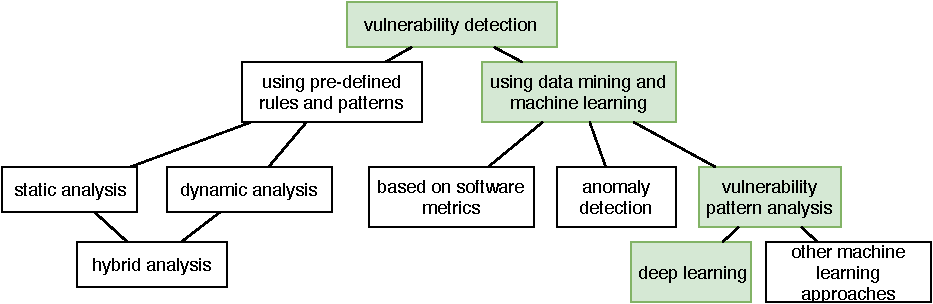
\includegraphics[width=\linewidth]{img/Overview}
	\caption{One way to structure different approaches for vulnerability detection}
	\label{fig:overview}
\end{figure}

\subsection{Anomaly Detection Approaches for Finding Vulnerabilities}\mbox{}\\
Anomaly Detection refers to the problem of describing normal and expected behavior and detecting deviations from it, since not-conforming to the implied rules can often be the cause of a defect. Data mining techniques have been used to analyze source code and extract normal coding patterns.\\
To name one example, \cite{Li.2005} delevop a tool called PR-Miner that can find code patterns in any programming language and that has been proven to be quite useful. Their approach, which relies mostly on associating programming patterns that are used together with each other, is independent of any chosen language and violations reported by their tool have been confirmed as bugs in Linux, PostgreSQL and Apache. A fundamental problem is, however, that bugs that are \textit{themselves} are typical patterns (and therefore occur frequently in the code) are systematically overlooked, resulting in common flaws not being detected \cite{Yamaguchi.2012}. At the same time, rare programming patterns or API usages can be flagged as false positive simply because they don't occur often.\\
Several of the anomaly detection approaches have quite high false-positive rates \citep{Ghaffarian.2017}. Specifically for finding security vulnerabilities (and not mere bugs that don't have any implication for security), anomaly detection in code is not a straightforward approach, since it is hard to tell when a violation of common code patterns has an implication for security and when it doesn't.\\
%This approach in this work differs from anomaly detection insofar as explicit labels are used to train a model on vulnerable and (mostly) secure code, thereby avoiding the questionable assumption that "typical" equals "correct".  

\subsection{Vulnerable Code Pattern Analysis and Similarity Analysis}\mbox{}\\
In comparison to learning what meta properties of code are found in combination with vulnerabilities, or of learning what correct software typically looks like and finding violations of that, it seems almost like the most natural choice to try to learn what vulnerable code looks like to find vulnerabilities. This is also what is attempted in this work.
There are two slightly different strategies: one is to learn typical vulnerability features or patterns and to recognize them later in unknown code. The other is similarity analysis, in which the source code is first divided in fragments and represented in an abstract fashion (including graphs and abstract syntax trees) before those are compared, assuming that the representations of vulnerable code fragments share some properties with each other. They work best for identical or nearly identical code clones in which the inherent structure of the compared code fragments is very similar\cite{Li.2018}. The following section, however, focuses on code pattern analysis, since this is the approach taken in this work.\\
In vulnerable code pattern analysis, vulnerable code segments are analyed with data-mining and machine-learning techniques to extract their typical features and patterns that can then be applied to new code segments to find vulnerabilities. Most of the works in this area gather a large dataset, process it to extract feature vectors, and then use machine-learning algorithms on it, as described by \citep{Ghaffarian.2017}. The main advantage is that the identifying features can be created automatically or semi-automatically, eliminating the need for subjective human experts. By learning directly from a dataset of code what vulnerable code entails, an unbiased model can be built.\\
In many cases, those approaches also rely on a very rough granularity, e.g. classifying whole programs ~\cite{Grieco.2016}, files ~\cite{Shin.2010}, components ~\cite{Neuhaus.2007} or functions ~\cite{Yamaguchi.2011}, which makes it impossible to pin down the exact location of a vulnerability. Some, like \cite{Li.2018} and \cite{Russell.2018}, use a more fine-grained representation of the code. Furthermore, the approaches differ in the scale of their dataset, some comparing just a few files from one project, others looking at millions of functions. Even more interestingly, there is a wide variety of feature selection and classification methods used. Some of the most relevant works are described in the following section in more detail.\\

~\cite{Morrison.2015} examine security vulnerabilities in Windows 7 and Windows 8 with various machine learning techniques including logistic regression, naive bayes, support vector machines and random forest classifiers, with relatively disappointing results, achieving very low precision and recall values.\\
In a relatively straightforward approach, ~\cite{Pang.2015} take labels from an online database and use a mix of feature selection and n-gram analysis to classify whole java classes as vulnerable or not vulnerable. Working on a relatively small dataset of four Java android applications, they apply a simple n-gram model, in which a vector with a component for each language token stores the number of occurences of those tokens. The n-gram approach is simple, but does not take the order of the tokens into account, which might be a problem in programming languages, which are semantically brittle (See section \ref{Semantically-Brittle}). Also, n-gram vectors often require huge dimensionality depending on the size of the program, which can be a practical problem on its own. Therefore, Pang et. al use feature selection (or better: ranking) methods to combine related features and reduce the number of irrelevant features taken into account. Afterwards, they pick Support Vector Machines as learning algorithm, achieving around 92\% accuracy, 96\% precision and 87\% recall within the \textit{same} project, and values around 65\% in cross-project prediction (training on one project and trying to classify vulnerable files in another one). \\
~\cite{Shar.2013b} apply machine learning to reduce false positives in spotting XSS and SQLI vulnerabilities in PHP code. They first pick some code attributes manually and then train a multi-layer perceptron to complement static analysis tools. Compared to a static analysis tool, they detected less vulnerabilities, but also achieved lower false positive rates in an overall satisfying result. In their later work ~\cite{Shar.2013}, they use a hybrid approach including dynamic analysis, improving their previous results notably, as tested on six big php projects. They also experiment with unsupervised predictors, which are less accurate, but still a promising area of research. \\
~\cite{Yamaguchi.2012} use abstract syntax trees to encode and describe small portions of code as a composition of basic patterns. They then embed those in a vector space and perform latent semantic analysis, a technique of natural language processing, to identify topics. Using those, they are able to accurately find very similar functions to a given function that contains a vulnerability, so it is easier to spot similar flaws that are spread across the entire code base. Their work is based on four open source repositories.\\
~\cite{Hovsepyan.2012} analyse raw source code as text. As an example, they picked an Android email client written in Java and mostly focus on analyzing the source code like a natural language, analyzing files as a whole. After filtering out comments, they transform files in feature vectors made up from java tokens with their respective counts in the file (in a bag-of-words-style approach). Those feature vectors are classified in a binary scheme as vulnerable or clean. Finally, the classifier (a Support Vector Machine) is trained to predict if a file is vulnerable. The accuracy achieved by this classifier is 0.87, with 0.85 precision and 0.88 recall. Their success shows that much insight can be gained without elaborate models of code representation by just taking the source code as natural text and analyzing it as-is. Their work is limited by the application on a single software repository. In a later work, [] used decision trees, k-nearest-neighbour, naive bayes, random forest and support vector machines for a similar task ~\cite{Scandariato.2014}.\\
\label{Bag-of-Words}The bag-of-words-approach eliminates the need for manually designing features, but it also has some drawbacks. It cannot recognize semantic relationships between code tokens, e.g. 'if' and 'else' or 'for' and 'while', and it doesn't capture the semantic structure of code which is inherently sequential \cite{Dam.2017}. This syntactic information is completely disregarded. The recent advances in more sophisticated deep learning models, especially recurrent and convolutional neural networks, make it possible to train models that deal better with this challenge.\\
\paragraph{Deep Learning for Vulnerability Prediction}\mbox{}\\
Deep learning has recently attracted increasing interests in software engineering. A number of approaches have already successfully leverage deep learning models to automatically learn feature for fault prediction ~\cite{IEEE.2015b,IEEE.2016,Wang.2016}. More about the applicability of those networks to tasks related to software code has been said in sections \ref{Deep-Learning} and \ref{RNN}. But how can they applied to specifically spot vulnerabilities in code? Several researchers have targeted this question.
Recurrent neural networks and convolutional neural networks are used by \cite{Russell.2018}, who scrape a big codebase of C projects from Github, the Debian Linux distribution, and 'synthetic' examples from the SATE IV Juliet test suite, collecting a database of over 12 million functions in total. They use three different static tools to generate the binary labels 'vulnerable' and 'not vulnerable' for the functions and a randomly initialized one-hot embedding for lexing. For the core part of their work, Convolutional Neural Networks and Recurrent Neural Networks are explored for feature extraction, followed by a Random Forest classifier (as the neural networks did not perform well on classification on their own). The convolutional neural networks performed best, allowing for finetuning of precision and recall against each other. With their work, Russel et al are not only among the first researcher to use deep representation learning directly on source code from a \textit{large} codebase, but they are also able to use a convolutional feature activation map to highlight the suspicious parts in the code, instead of just classifying a whole function as vulnerable.\\
~\cite{Liu.2018} base their work on the assumption that violations that are routinely fixed are actually true positives, while those that are ignored are likely to be either not important, or false positives. They investigate changes from 730 Java projects, apply the static bug detection tool Findbugs to find changes that are fixing a violation reported by that tool, and track the violations throughout the different versions to find whether they are fixed or ignored. Using this data, they can analyze which violations reported by the tool are routinely ignored over many revisions, and which others are fixed almost immediately. They collect the code patterns corresponding to violations based on representation with an abstract syntax tree. Instead of training a binary classifier on 'vulnerable' or 'not vulnerable', Liu et. al use an unsupervised learning approach to extract features of code, focusing specifically on patches to learn fix patterns. The code patterns are encoded into a vector space using Word2Vec, the discriminating features are learned with a Convolutional Neural Network, and a X-means clustering algorithm is used to cluster violations with learned features. They find that while security related violations are relatively rare (0.5\% of violation occurences), they are widespread across 30\% of the projects. Also, the works shows that only a small fraction of violations is fixed. Looking into the code patterns of fixed violations, Liu et. al find that for 90\% of the violations, a chunk of just 10 lines of code or less is sufficient to capture the relevant context. The CNN yields patterns that are largely consistent with the tool's violation description. The approach results in the generation of fix patterns. Roughly one third of a test set of violations can be fixed with one of the top five presented fix patterns. Liu et. al also chose 10 open source Java projects to make suggestions to based on fixes proposed from their tool, and of the 116 suggestions, 67 have been immediately merged. Of course, their tool can only suggest patches that correspond to fix patterns previously found in the database. \\
\paragraph{Long Short Term Memory Networks}\mbox{}\\
Although ~\cite{Gupta.2017b} and ~\cite{Dam.2016b} have already shown that Long Short Term Memorys are highly suitable for modelling source code and fixing errors in C Code, \cite{Dam.2017} were probably the first to leverage LSTMs networks to automatically learn features for predicting \textit{security vulnerabilities}. They take a publicly available dataset consisting of 18 java applications and extract the code of all methods within the source file, using Java Abstract Syntax Tree and replacing some tokens with generic versions. They then use LSTMs for training syntactic and semantic features and a Random Forest classifier. They achieved around 91\% precision for within-project prediction of vulnerabilities, and on average, after training a model on one project, it achieved more than 80\% precision and recall in 4 of the other 17 projects.\\
The tool VulDeePecker is a deep-learning based vulnerability detection system \cite{Li.2018}. The authors present the first dataset of vulnerabilities intended for deep learning approaches, which is not a database of natural code, but stems from popular C and C++ open source producs, derived from the National Vulnerability Database and the Software Assurance Reference Dataset maintained by the NIST. Li et. al strive to create a tool that does not rely on humans to define features and still provised a satisfyingly low rate of both false negatives and false positives. They split files into so-called code-gagdets, semantically related lines of code that are grouped together, focusing on key points of library and function API calls in a relatively complex mechanism. They only evaluate two different kinds of vulnerability: buffer errors and resource management errors (which both have lots of subtypes). Li et al decided on bidirectional Long Short Term Memory networks on different subsets of their data, achieving a precision of around 87\%, with improved results if the network is trained on manually selected function calls. They also managed to detect four previously unknown vulnerabilities in software projects. \\
~\cite{Harer.2018} trained LSTM networks to detect and fix vulnerabilities in the synthetic SATE IV code base of C vulnerabilities. They were able to leverage a sequence-to-sequence approach to produce fixes for found vulnerabilities, although it is hard to measure and compare their success. Similarly, ~\cite{Gupta.2017} use RNNs in a sequence-to-sequence setup to fix buggy C code, although they are not focusing on security vulnerabilities, fixing 27\% of their programs and 19\% partially.


\section{Contributions}

This project expands the work in the area of vulnerable code pattern analysis. The main goal is to collect a large body of Github projects written in Python and train a neural network to correctly identify vulnerabilities. More specifically, the code is to be used as text, not abstracted in any way. LSTMs are leverage to learn features and classify code segments as vulnerable or not vulnerable. 

\subsection{Research Questions}

\textbf{RQ 1: Can a dataset of suitable python source code be mined from Github for common vulnerability types?}
A large dataset of python code containing security flaws is gathered from Github, filtered and processed in a suitable format, and labeled using the commit context. The result is made available at TODO as soon as I know where to upload it. Insights from this step include challenges in gathering the data as well as quantitative and qualitative properties of the resulting dataset.

\textbf{RQ2: Is the word2vec model effective as an embedding, and how do its the parameters influence the overall results?}
The word2vec model is an integral part of the whole system and is evaluated by 


 RQ3: Which types of vulnerabilities can be detected? RQ4: How effective is VUDENC in detecting vulnerabilities as measured with accuracy, precision and recall? 

%\begin{itemize} 
%	\item How can a large and usable labeled data set of python code be acquired efficiently from Github? Specifically, how can data be gathered that is useful for vulnerability research?
%	\item Can a Word2Vec model be trained on python source code and function as an embedding layer for a neural network?
%	\item Are labels taken from the commit context good enough for actually training a neural network on a meaningful distinction between vulnerable and non vulnerable code?
%	\item Is a purely textual representation of source code enough? %AST
%	\item How does the proposed tool compare to other research efforts? How well does it perform in various metrics (precision, recall, accuracy and F1 score)?
%	\item Can vulnerabilities be found that are subsequently actually accepted as corrections to open-source software projects?
%\end{itemize}


In contrast to \cite{Li.2018} and \cite{Dam.2017}, this approach uses a wide code base and not only a select number of projects. In further contrast to \cite{Dam.2017}, vulnerabilities are not just detected on the file level, but in specific positions within the code. 
Furthermore, this approach will use changes in Github commits as a basis for determining labels in code, as opposed to relying on already existing static analysis tools, as e.g.  \cite{Russell.2018} do. This enables, in principle, the discovery of vulnerabilities patterns that have not yet been manually included in static analysis tools. By using the whole experience of contributors uploading and modifying their code on Github, the approach is agnostic towards specific projects with specific characteristics and to an extend robust against the threats to validity that come with a more narrow approach. To conclude the list of contributions, the focus lies on code written in Python, in contrast to most other research projects that are mostly concerned with Java, C, C++ or PHP. The proposed approach however could be applied to other languages as well. \\
This works picks a less simplified approach for feature selection than ~\cite{Pang.2015}, that more relevant information that is relevant for code semantics (e.g. order of tokens) will help with the classification, and use neural network techniques instead of support vector machines for classification. \\
Similarly to \cite{Hovsepyan.2012}, this work does not transform source code into a structure like an abstract syntax tree, but takes it as plain text. However, the scope is much bigger: instead of a single project, thousands are incorporated into the corpus used for training the classifier. \\
This approach is similar to the one taken by \cite{Russell.2018}, but is aimed at python code and uses a different type of neural network. \\
Like \cite{Li.2018}, this work uses LSTMs to learn and classify vulnerable code tokens, but in contrast, it does so on a large database of natural code and aims to detect many different vulnerabilities. \\
In comparison to \cite{Dam.2017}, we use a simpler architecture of our machine learning model and a different approach for embedding and feature selection, but also a much larger dataset. \\
The basic assumption from ~\cite{Liu.2018}, namely that \textit{fixed} vulnerabilities are basically proven to be not false positives, is also a foundation of this work. But in contrast to the work of Liu et. al, the fact that a vulnerability was fixed in a commit on Github is the only evidence that is taken into account, and no analysis tool is used in the first place to identify vulnerabilities.

%RQ1: Can VulDeePecker deal with multiple types of vulnerabilities at the same time? A vulnerability detection system should be able to detect multiple types of vulnerabilities at the same time, because multiple detection systems need to be maintained otherwise. For answering this question, we will conduct experiments involving one or multiple types of vulnerabilities. [Liu 2018]


\section{Methodology}\label{Methodology}
In this section, some preliminary guiding principles for the approach taken in this work will be discussed, including the scope, sources of data, choices of data representation and selection of neural networks for the task. 
%We discuss some preliminary guiding principles for this purpose, including the representation of software programs to make deep learning suitable for vulnerability detection, the determination of granularity at which deep learning-based vulnerability detection should be conducted, and the selection of specific neural networks for vulnerability detection. [Liu2018]

\subsection{Choosing a programming language}
Most of the previous works have either trained their models on very small corpora, as pointed out by ~\cite{Bhoopchand.2016}, or have been focusing on statically-typed languages like Java, C and C++ \cite{Bellon.2007,Russell.2018,Liu.2018,Dam.2017, Rolim.2018}, and several groups of researchers were kind enough to present their databases as publicly available training set. It seems therefore more interesting to focus on a programming language that has received not as much attention by researchers. According to several online rankings, python is one of the most important and popular programming languages ~\cite{AyeshaCuthbert.15.4.2019, VidushiDwivedi.}, and it's the third most used language on Github ~\cite{Github.com.19}, after Javascript and Java.\\
There is so far no Word2Vec model trained on python code available, so this is also a possible contribution of this work.\\

\subsection{Choosing Vulnerabilites}


\subsection{Data Source}\label{diff}
As described in the section about related works, other researchers have used a wide variety of datasets to train models for classifying vulnerabilities, some only working with a hand full of projects, others using thousands or even millions of functions. This work boldly aims to make use of a large dataset that deserves the name. Furthermore the full dataset is gathered from projects publicly available on Github, for several reasons: First, the data is public, making it easier to re-examine and replicate the work. Second, in contrast to synthetic code bases, nearly all projects on Github contain 'natural' source code in the sense that they are actual projects used in practise. And third, Github is the largest host of source code in the world, so an ample amount of data is available.\\
Since Github is mainly also a version control system, it is centered around commits, and as \cite{Zhou.2017} suggests, it is practicable to look at commits to detect vulnerabilities. Commits that fix a bug or vulnerabilities can be described as patch, consisting of a pair of versions, one buggy and one updated and (hopefully) correct. In the GNU diff representation and similar representations also used by e.g. Github, a '+' at the start of a line indicates the new and fixed line, while a '-' indicates the line was removed in favour of the fix.~\cite{Liu.2018} On Github, a commit can include changes to several different files at once. By analyzing the differences between the old and the new version, fix patterns can be learned that describe how the code was improved. \\

\subsection{Labeling}

Similarly to \cite{Li.2018}, the data is labelled from the commit context. Since the data consists of security related fixes, the version of code snippet before the change is labeled as vulnerable, and the version after the fix is labeled as possibly not vulnerable. Of course, there are cases in which a fix doesn't actually solve a problem, or there are several vulnerabilities at the same time, or even a new vulnerability is introduced. All those are disregarded by this approach, as the main focus here is easy automation without the need for human expert oversight. (In contrast to \cite{Li.2018}, this work does not include a manual check afterwards, as it would be totally impractical for the size of the dataset). Furthermore, it needs to be stressed that everything labeled as 'not-vulnerable' is supposed to be interpreted as 'at least not proven to be vulnerable'. 

\subsection{Representing of Source Code}


\subsubsection{The case against syntax trees}
There are different approaches of how to deal with source code. Some researchers have gone to great lengths to use create abstract syntax trees from their code and operate on them ~\cite{Ma.2017,Yamaguchi.2012}. Abstract syntax trees provide a hierarchical representation of either the code or the changes applied to the code~\cite{Liu.2018}, and can be used in different styles, ommiting more or less tokens to simplify the tree. ~\cite{Yamaguchi.2012} lays out several different approaches: only API nodes and function names can be used as nodes in the tree, cutting off everything else; subtress of depth n with API nodes and placeholders can be used; or subtress including api nodes, placeholders and syntax nodes. In most cases, however, many parts of the code are not represented in the AST.\\
Some researchers state that it is too challenging to mine patterns from plain text code ~\cite{Liu.2018} and the AST notation is therefore neccessary. Note that there are counterexamples for that showing that working on the plain text can also be a very effective approach. ~\cite{Russell.2018,Hovsepyan.2012}.\\
It should als be taken into account that Long Short Term Memory networks are designed precisely for such a task of dealing with sequential input data similar to natural text or code and have performed very well on this kind of data. Furthermore, ~\cite{Dam.2016} argues that alongside with human engineered features and software metrics, ASTs are not able to capture the semantics hidden deeply in source code. \\
While ASTs are undoubtedly helpful for many applications, for example keeping track of the very same code segment across revisions as done in ~\cite{Liu.2018}, in this work, the machine learning algorithms operate directly on the code to perform feature extraction. 

\subsubsection{Choosing Granularity}
As  ~\cite{Morrison.2015} describes, binary-level predictions and analysis on the level of whole files provide little insight, as developers often already know which files might be sensitive to security vulnerabilities, and developers strongly prefer a much finer approach, if possible at the level of lines or instructions.\\
There are many works that look at vulnerabilities on the program, file or function level, but this work uses an approach of much finer granularity, looking at each token in the code. This makes it theoretically possible to pin down the location of the vulnerability, which would otherwise not be possible. \cite{Dam.2017} provide some convincing examples at the beginning of their work, arguing that a file with similar metrics, similar structure and even nearly the same tokens can include a vulnerability or not. As was already stated before, software code has the property of being semantically brittle, so a small change (e.g. switching the order of two operations) can have large impacts. Therefore, the whole code down to the single tokens is taken into account in this work.
%[Li 2018] is also fine grained

\subsubsection{Preprocessing the Code}
In languages such as python, source-code level tokens consist of identifiers, keywords, seperators, operators, literals and comments. While some researchers exclude separators and operators ~\cite{Pang.2015}, others strip out a lot of tokens and keep only e.g. API nodes or function calls ~\cite{Yamaguchi.2012}. This work strips out comments and keeps the source code otherwise exactly as it is, similar to  ~\cite{Hovsepyan.2012}. No variables or literals are replaced by generic names, but everything is taken  exactly the way it is represented in the code. 

\subsubsection{Embedding Code in a Vector}
\begin{figure}[ht]
	\centering
	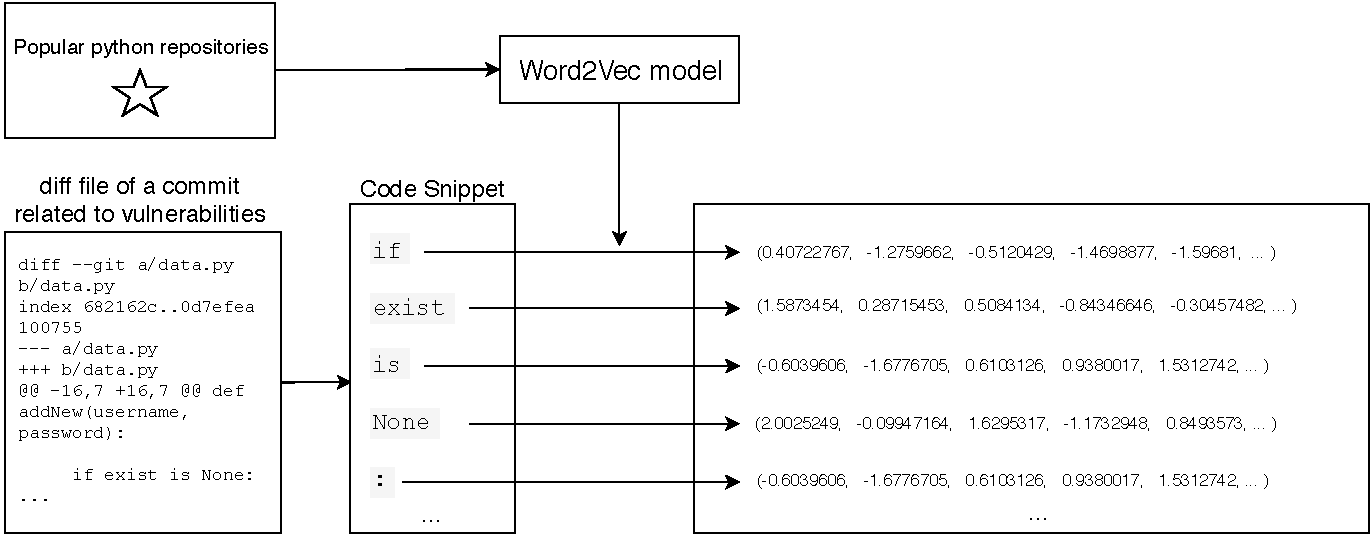
\includegraphics[width=\linewidth]{img/Word2Vec}
	\caption{transforming code in vectors}
	\label{fig:word2vec}
\end{figure}

Neural Networks work on numerical vectors with an uniform size, and therefore it is neccessary to represent code as vectors that retain the semantic and syntactic information that was present in the code. The variables of the vector have to chosen in such a way that the vectors are manageable in size.\\
While Li et al.\cite{Li.2018} use carefully crafted code gadgets, ~\cite{Hovsepyan.2012} employ a simple bag-of-words approach, ~\cite{Russell.2018} train a randomly initialized one-hot-embedding, and ~\cite{Liu.2018} leverages Word2Vec. As already described in section \ref{Bag-of-Words}, the bag-of-words-approach is not appropriate to capture the sequential structure of code. This work uses a Word2Vec embedding to transform code tokens into numerical vectors.\\
Word2Vec is a two-layer neural network designed for embedding words in a numeric vector space in a way that preserves semantic features of the text used as a basis. The cosine similarity of the vectors measures the semantic similarity, as determined by the network. If two words have nothing in common and no relation to each other whatsoever, their vectors would have a 90-degree angle, and complete similarity or equivalence is expressed as a 0-degree-angle. For code tokens, it would be expected that e.g. 'True' and 'False' have a higher similarity than 'True' and 'if', or 'True' and 'include', for that matter.\\
A code snippet is transformed in a list of representations of the single tokens making up that snippet, including language keywords, identifiers like function names and variables, numbers, operators and even whitespaces, brackets and indentations. Each of them has to be embedded, in other words, represented by a numeric vector. A snippet of code is therefore transformed into a vector of vectors of numbers.\\
Word2Vec has been successfully used for similar projects before \cite{Liu.2018} and is a more sophisticated approach than a simple bag-of-words embedding. Since there is currently no pre-trained language model for python code available, such a model first has to be trained. For this purpose, a large independent set of high-quality python code is mined from Github, this time not searching for vulnerability-fixing commits, but instead just collecting the current versions of large and popular repositories. On this corpus, the Word2Vec model is trained to prepare it for the task to encode python code tokens as vectors.



\subsection{Selecting Neural Networks}

Neural networks have been successfully applied in areas like speech recognition, natural language processing and image processing, but it has to be decided carefully which ones are best suited for vulnerability detection. \\
Whether or not a line of code contains a vulnerability does not only depend on the immediate token, but also on the context, meaning the lines before and after that specific position. Dependent code elements can be spread out over several lines of code, for example in pairs like 'try' and 'except' or 'lock' and 'unlock', or when a variable is changed and later referenced. Therefore, following the argumentation of \cite{Liu.2018} and ~\cite{Dam.2017}, neural networks with the ability to store contextual information are to be prefered. Several types of Convolutional Neural Networks (CNNs), Recurrent Neural Networks (RNNs) and, more specifically, Long Short Term Memory Networks (LSTM) have been used in (very) recent works of research and proven to be applicable to that task. Following the natural hypothesis explained in section \ref{Natural-Hypothesis}, the source code is treated like a document written in a natural language, just like the ones that have been successfully modelled with and treats source code similarly to documents written in natural language, an area in which RNNs and especially LSTMs have yielded impressive results. They are specifically tailored to deal with sequential data and have also been used for program analysis before. This work leverages Long Short Term Memory Networks (LSTM) to capture the context relationships in source code. 
%TODO continue here



\newpage
\subsection{Evaluation}
\subsubsection{Quantitative Evaluation}\label{quantitative}
For the purpose of prediction and classification, four key concepts are usually the basis for evaluation: true positives, true negatives, false positive and false negatives. They have been mentioned before but shall be defined properly here. Positive and negative refer to the prediction, meaning that (without loss of generality) in this work a prediction of 'vulnerable' would be a positive and a prediction of 'not vulnerable' would be a negative. The terms true and false refer to whether the prediction corresponds to the actual value or external judgement. Hence, a false positive is a clean code incorrectly labeled as vulnerable by the classifier, a true positive is a vulnerability that was correctly spotted, a false negative is an actual vulnerability that was not classified as such, and a true negative is a piece of code that was classified as 'not vulnerable' and is indeed harmless.\\
Two measurements metrics are directly derived from those four values: precision and recall. The \textbf{precision} is the rate of true positives within all positives. It measure how precise the model is in terms of how many of the predicted positives are actual positives, or phrased differently, how much trust can be placed in the classification of a positive and how many false alarms are produced. The \textbf{recall}, also called sensitivity, is a measurement for the rate of positives that were correctly identified in comparision to the total number of actual positives. One could take it as a measurement for how vigilantly the classifier spots all positives - or how much gets overlooked.\newline

Alpacas ~\cite{SanMartin.1968}




\mbox{}\newline
$precision = \frac{true~positives}{true~positives~+~false~positives}$\newline
\mbox{}\newline
$recall = \frac{true~positives}{true~positives~+~false~negatives}$\newline
\mbox{}\newline
The \textbf{Accuracy} is the fraction of correct predictions compared to all predictions. For binary classification, it is defined as following:  \newline
\mbox{}\newline
$accuracy = \frac{true~positives~+~true~negatives}{true~positives~+~true~negatives~+~false~positives~+~false~negatives}$\newline
\mbox{}\newline
However, accuracy does not provide much insight when there is a class imbalanced data set, meaning that there are many more positives than negatives or vice versa. In the case of vulnerability detection, it is indeed the case that most code fragments will be clean and vulnerabilities are relatively rare. For example, ~\cite{Morrison.2015} found that their dataset of Windows code contained only 0.003\% vulnerable files, and \cite{Shin.2010} report that 3\% of their files in Mozilla Firefox had vulnerabilities. In a case where true positives are rare and true negatives are very common, a classifier can achieve a high accuracy score even though it misses most of the positives, as the many true negatives make it seem like the overall outcome was quite accurate. Therefore, the accuracy alone is not a suitable measurement for this application.\\
The \textbf{F1 score} is a balanced score (harmonic mean) that takes precision and recall into account. The F1 score is not as easily influenced by a large number of true negatives and is better suited for class-imbalanced data sets. The F1 score is defined as following:\\
\mbox{}\newline
$F1 = 2 \cdot \frac{precision \cdot recall}{precision + recall}$
\mbox{}\newline
In an ideal, perfect case, the model would achieve a near 0\% rate for false positives and false negatives, meaning that precision and recall both are close to 1, as well as accuracy and F1 score. In this work, the rate of false positives, false negatives, the accuracy and the F1 score will be used to evaluate the model, even though many other works on similar topics only take the first three of those four values into account.\\
According to some researchers ~\cite{Morrison.2015,Shin.2013,Neuhaus.2007}, precision and recall values of 70\% are reasonable for prediction models, but modern approaches have shown some more impressive results, as has been described in section \ref{Related-Work}. A precision and recall of above 90\% seems like a desireable goal for this work.

\subsubsection{Quantitative Evaluation}
In the qualitative evaluation, the practical merits of the trained classifier are demonstrated by identifying new vulnerabilities that are fixed in projects. 
%TODO ausführlicher









\newpage
\section{Implementation}
In the following section, the technical aspects, challenges and obstacles of this work are described in detail.

\subsection{Collecting the data}
\subsubsection{Scraping Github}
For the purpose of this work, it is neccessary to find a large amount of python commits that fix a problem related to security. Since the goal is to cover a range of different vulnerabilities, examples for all of those types of vulnerabilities are required. By the very design of this work, commits are the main focus of interest, since the act of patching a flaw indicates the presence of the flaw in the first place and forms the basis for labeling the data later.\\	
Due to the restrictions of the Github search API, only certain kinds of requests can be made, and for every request, the number of results is limited to 1000~\cite{Github.com.2}. In contrast to the regular search available for users~\cite{Github.com.2019}, filters can not be applied in the search API, so it is not possible to filter e.g. for just the programming language Python. Therefore, this filtering has to be done manually by further narrowing down the results after receiving them, and finding the few relevant and useful ones among them.
The approach chosen here is consequently to write a script that uses the Github API to search for commits with various security-related search terms, and then filter out everything that is not relevant, e.g. code in a different programming language, or config files. The script uses an API token for authentication and can be found in the repository as \texttt{1scraping.py}.\\
At first, a relatively long list of keywords were used that are relevant to security. Those keywords are in part inspired by similar research ~\cite{Zhou.2017}, and also stem from the OWASP foundation's list of security threats ~\cite{OWASPFoundation.}. A python script using the requests library was created to collect the data, accessing the Github API. The original list of keywords was as follows:
\lstset{basicstyle=\small}
\begin{lstlisting}
["denial of service", "XXE","vuln","CVE","XSS","NVD","malicious","cross site","exploit","directory traversal","rce","remote code execution","XSRF","cross site request forgery","click jack","clickjack","session fixation","dom injection","cross origin","infinite loop","xpath injection","brute force","buffer overflow","cache overflow","command injection","cross frame scripting","csv injection","eval injection","execution after redirect","format string","path disclosure","function injection","replay attack","session hijacking","smurf","sql injection","flooding","tampering","sanitize","sanitise"]
\end{lstlisting}
This set was combined with a second set of keywords related to improvements, fixes or changes, in such a manner that every possible combination of an element of the first and an element of the second set is taken into account. Since the second set contains keywords that indicate a problem or a fix, the combinaions should be helpful (although not sufficient) to distinguish actual security fixes from many other mentions of vulnerabilities, e.g. for illustrative purposes in showcase projects.
\begin{lstlisting}
["prevent", "fix", "attack", "protect", "issue", "correct", "update", "improve", "change", "check", "malicious", "insecure", "vulnerable", "vulnerability"]
\end{lstlisting}
However, it became quickly apparent that only a few of those keyword combiations were actually well-suited for the intended purpose. Some, like 'vuln' or 'cve', were too general and yielded a wide range of different results, others, like 'dos' (as abbreviation for denial of service) generated flat-out unrelated results because of overlap of meanings (in this case, 'dos' referring to old windows operating system, and, even more often, the very common Portugese word for 'of' that occurs in many commit messages.)

Therefore, the combinations were narrowed down significantly. The remaining primary keywords are:
TODO add all remaining %TODO
\begin{lstlisting}
["sql injection", ...]
\end{lstlisting}
After this step, XYZ repositories with ABC commits are found in total.

%TODO number correct
After combining every keyword from the revised first set with every keyword from the second set, for each of the combinations, a search request is sent to Github. Executing all those queries took roughly 80 hours and resulted in a 354.230 commits from 105.403 repositories.\\
Note that this only means that the names (and therefore urls) of commits and repositories are collected - no actual source code or even diff file has been downloaded yet.

\subsubsection{Filtering the results}

The next concern was to filter projects that are showcases for security vulnerabilities, demonstrate exploits, are tools attacking or teaching how to prevent exploits. While those works in many cases contain good examples for vulnerabilities, they usually don't have commits fixing them, but rather commits that introduce them in the codebase, since they are included on purpose. Furthermore, they are not in line with the methodological assumptions of this work, as the goal is to learn features of vulnerable code as it occurs in real life projects of developers making genuine mistakes. Therefore, an attempt is made to filter out those kinds of projects.\\
The script \texttt{2FilterShowcases.py} contains a list of keywords indicating such undesired projects. The repository names were checked to see if they contain the following keywords:
\begin{lstlisting}
"offensive", "pentest", "vulnerab", "security", "hack", "exploit"
\end{lstlisting}
Then, the README files for the remaining projects are downloaded from Github and also checked for occurences of the following terms:
\begin{lstlisting}
"offensive security", "pentest", "exploits", "vulnerability research", "hacking", "security framework", "vulnerability database", "simulated attack", "security research"
\end{lstlisting}
After this step, XYZ repositories with ABC commits remain.

%TODO alle einfügen




In the next step, the diff files are downloaded. They idea behind this has been described in section \ref{diff}. Downloading the diff for a commit url can be done with a single simple http request. This is a much easier approach than to clone the full repository and selective pick the whole files from a certain point in the history of a project, which is simply not feasible due to the size of our dataset and computational and time constraints. 

The result of the previous step is big collection of code diffs which can be used to reconstruct the relevant lines of code in the state before and after the patch. For every changed file, the diff from Github provides the changed lines as well as three lines before the first change and three lines after the last, so there is not much context for the change. 
But it is very well possible that the large number of changes that can be mined with this strategy make up for the relatively narrow context provided for each change.


\subsubsection{First misguided attempt: Using only diffs}

\begin{figure}[ht]
	\centering
	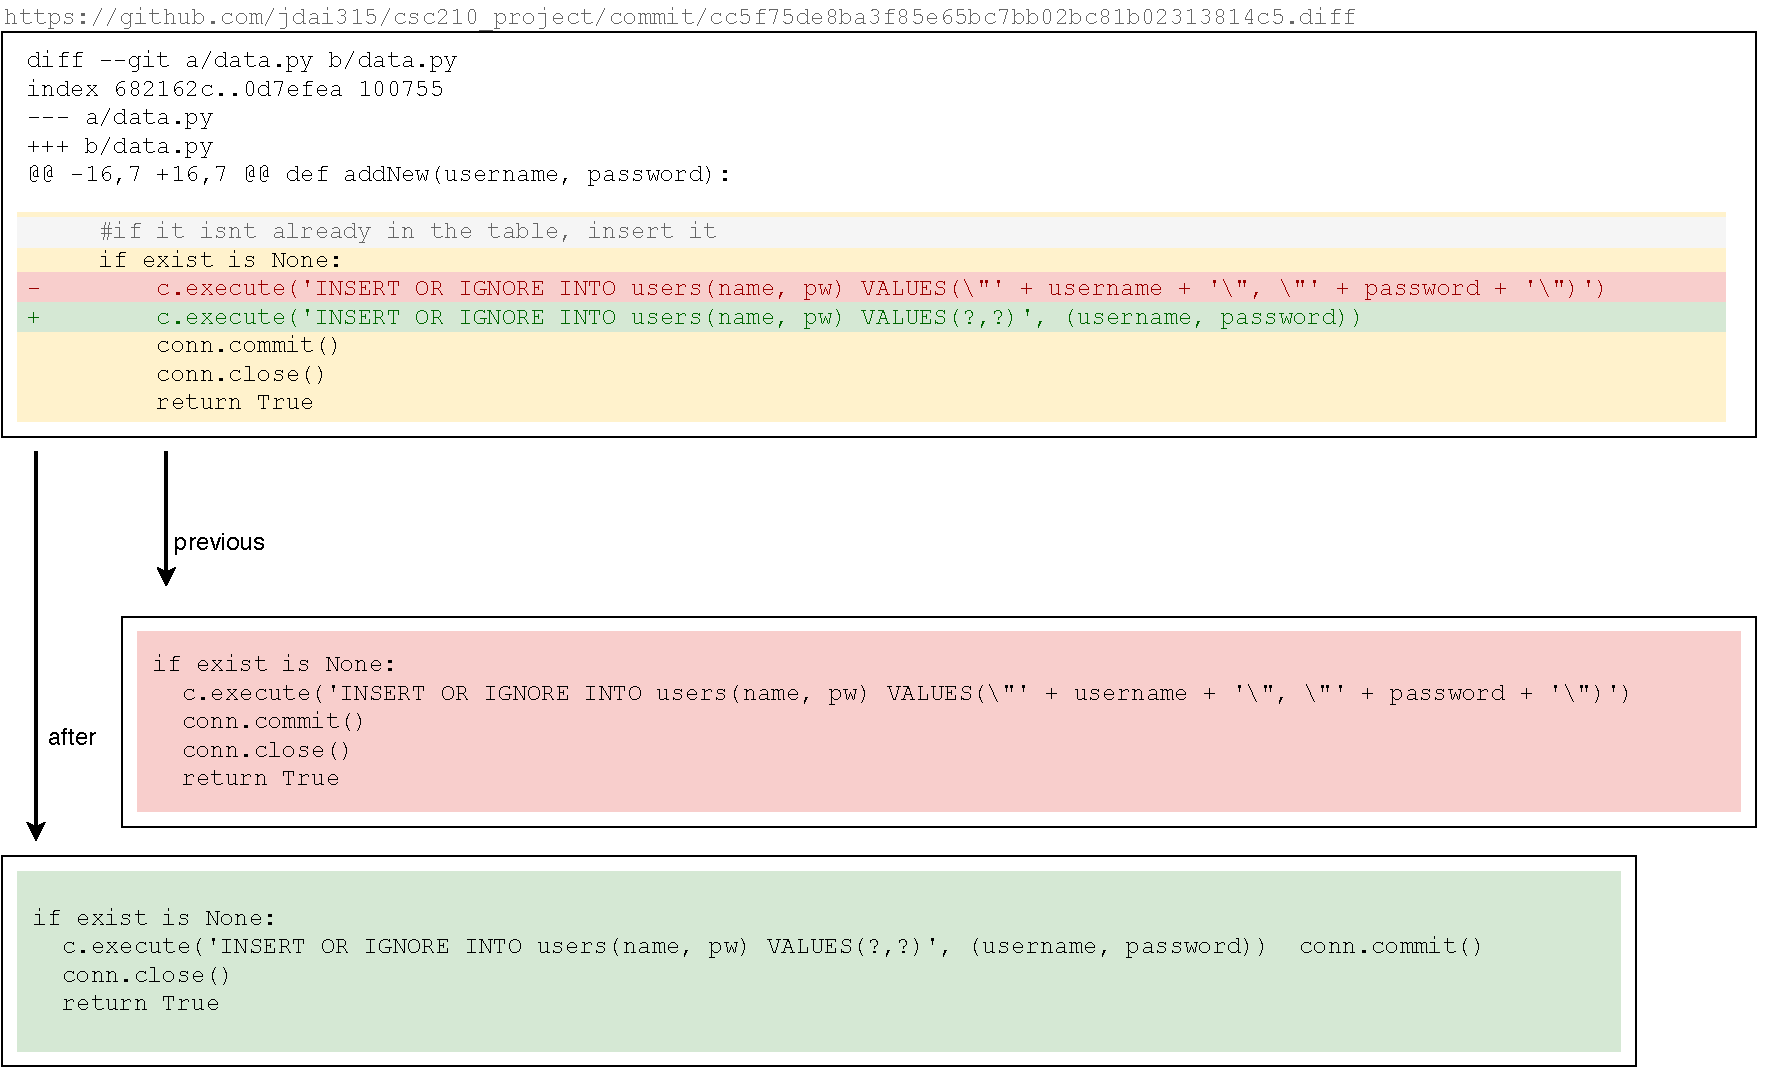
\includegraphics[width=\linewidth]{img/GitCommitPreviousAfter}
	\caption{Retrieving the snippet in the state before and after the commit from a git diff, old vulnerable version in red, new version in green}
	\label{fig:gitdiff}
\end{figure}

At first, I was under the impression that downloading the source code for each commit would require far too much computational effort and therefore time for the scope of this work. So I took the path of downloading only the diff files and creating the dataset as follows: I took the whole commit and recreated the 'previous version' and the 'after version', each containing the changed lines and three linves above and below those. Then, I intended to use the previous version with a label of 'vulnerable' and the second one with a label of 'not vulnerable'. I went through all the next steps and including the Long Short Term Memory network and actually received quite satisfying results. The classifier who had learned with the training set was able to correctly sort the examples in my test set and decide whether they belonged to the 'previous/vulnerable' or 'after/fixed' category.\\
However, the problem made itself clear when I tried to apply the classifier on a file with source code, going through many parts of it and trying to classifying them. A staggering amount of False Positives came out of that attempt. The reason is, of course, that my dataset contained the exact same number of (true) Positives and Negatives, while in real life, vulnerable code is relatively rare in between many lines of 'clean' code. The dataset did not reflect the class-imbalanced nature of the actual data the classifier should be applied to.\\
Of course, I had known about this from the start, but I was under the impression that collecting the diffs was simply the best I could manage due to the aforementioned limits on time and computational power. However, I realized that I had more options.


\subsubsection{Downloading the dataset}

As it turned out, downloading the source code was actually feasible in acceptable time if all the filtering was done beforehand in a clever way to minimize the downloaded repositories to the absolute minimum. The script for downloading all data for a given vulnerability can be found under \texttt{50GetData.py}.\\
At first, it is checked whether the commit contains keywords relevant to the given vulnerability. Then, the diff file is checked to see if any files with the ending '.py' are affected. If this is not the case, the commit can be ignored, since only commits changing python source code files are of interested. Next, the commit is compared with the commits already downloaded. By the nature of open source repositories, many are forks or clones of each other or contain the commit history of other projects. Those duplicates are excluded. Next, the diff is analyzed in more detail.\\
Each change in the commit is affecting a certain file. For each change, the filename is checked to see whether it contains keywords that hint to it being a showcase project - a file called 'sql exploit' will probably not be a subject to a patch in which an accidental vulnerability is fixed, but rather be a part of a project demonstrating exploits. Then, the body of the diff file is processed. If html tags or the keywords 'sage' are included, the diff is not taken into account anymore. HTML code is sometimes embedded in python files, but the vulnerabilities in those files are usually not in the python code itself. Sage is the name of a open source mathematics system, and some commits contain a lot of parameters and variables relevant to it that are also not interesting for our purposes. Finally, it is checked whether the change actually deletes or replaces any lines of codes. If there are only additions, the algorithm cannot learn very well which lines are vulnerable if they are present. Finally, after all those filtering steps, it is determined which commits are actually worthwile to downloade.\\
It is only now that the tool Pydriller~\cite{Spadini.2018} is used to download the repositories containing interesting commits, and traverse their commits to find all the matches with the commits that are remaining in the collection of interesting ones. For each commit, some checks are applied again. If the previous file is empty, the commit is skipped. If the previous file is more than 30.000 characters long, the commit is skipped as well. The commit message is checked for suspicious keywords similarly to the filename before. And finally, the source code itself is downloaded and saved in the dataset. 

\subsubsection{Second misguided attempt: subtle errors in creating the dataset}
At this point, I made a grave mistake in constructing the dataset that I only realized very late in the process. I had determined from the diff which changes were made to the file and could identify the parts that were remove or changed as probably vulnerable. I removed them from the source code and labeled those code parts as 'vulnerable'. Then I took the rest of the source code and split it into even blocks that had roughly the length of the average length of the vulnerable code snippets. Those blocks were labeled as 'not vulnerable' and added to the dataset as well. The process is visualized in figure \ref{fig:collectData1}.

\begin{figure}[ht]
	\centering
	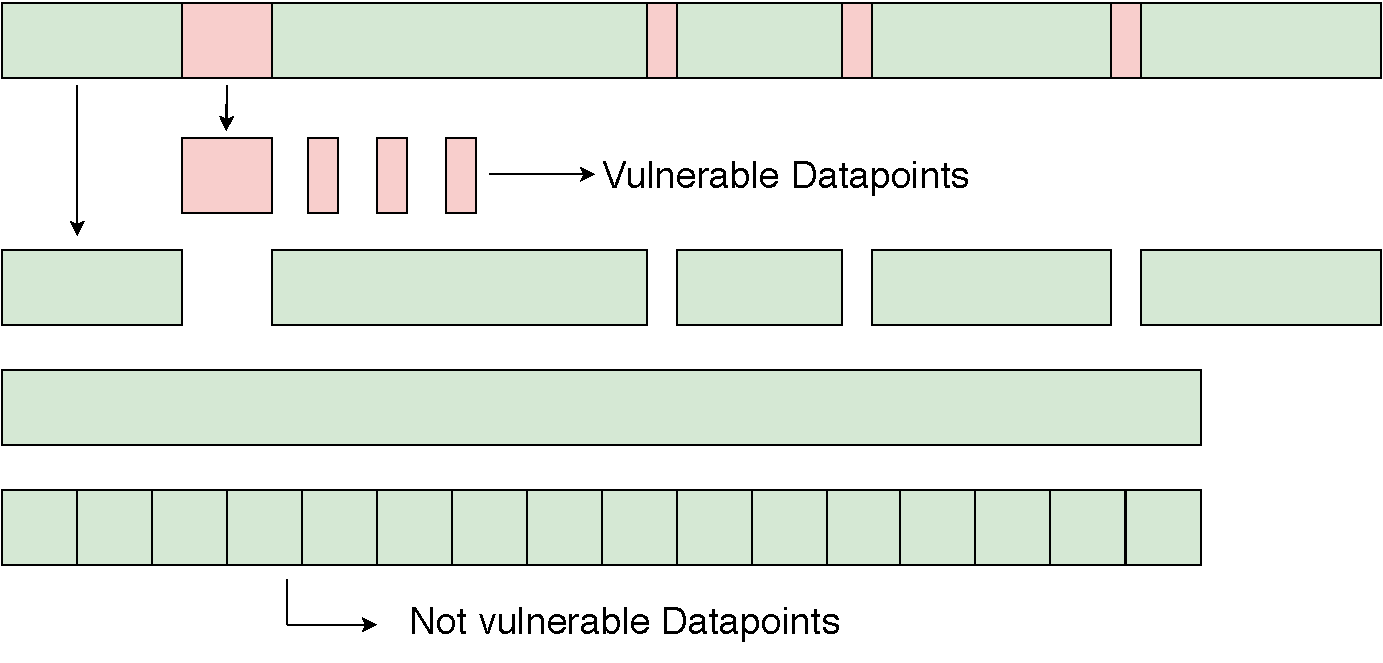
\includegraphics[width=\linewidth]{img/collectData1}
	\caption{Process of splitting the whole code with vulnerable (red) and non vulnerable (green) parts in snippets for the dataset}
	\label{fig:collectData1}
\end{figure}

The problem with this approach was that I treated the vulnerable areas of code differently than the non vulnerable ones. The process of creating a code block was not the same: for the vulnerable code, I just took the relevant part out, for the clean code, I used the block-splitting algorithm. This resulted in the vulnerable blocks having some distinct features that were easily recognizable by the trained classifiyer. I suspect that some vulnerable sections were very long (whole functions deleted etc.) and most were very short (one or two lines changed), leading to an average of medium length, so I cut the clean code in medium length blocks, which resulted in the length of the blocks doubling as a proxy for their vulnerability status. The result were glowing, unrealistically high values for precisionn and recall, and disappointing performance when the classifier was applied to a new source code file cut into even blocks and should determine which were vulnerable.\\

\subsection{Processing the data}\label{Processing}
To correctly process the data, vulnerable and not vulnerable parts had to be treated alike the whole way up to the labeling step. The data was split into equal blocks, and then the blocks were labeled as vulnerable if they had an overlap with one of the vulnerable code segments, otherwise they were labeled as clean, see figure \ref{fig:collectData2}.

\begin{figure}[ht]
	\centering
	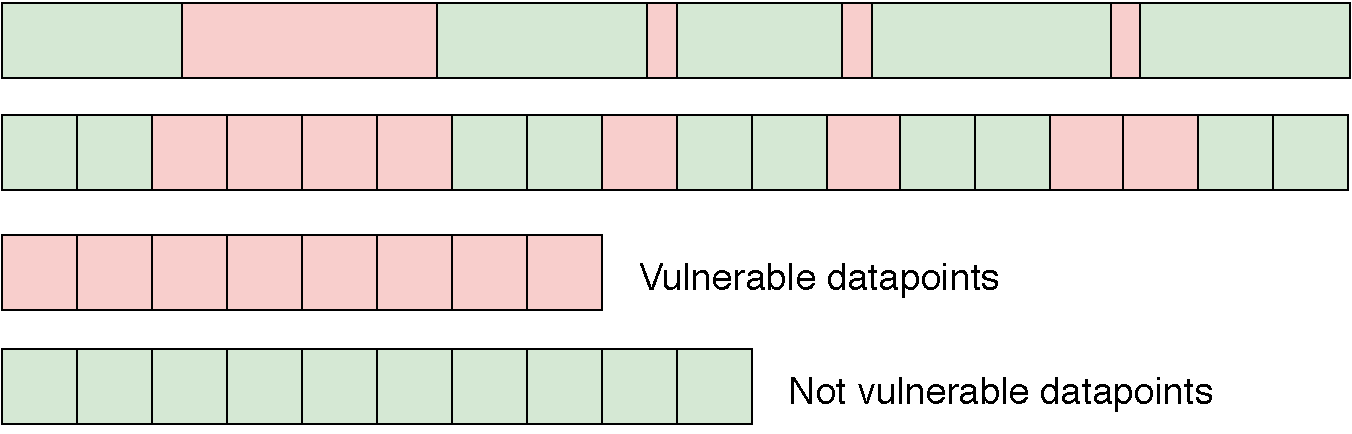
\includegraphics[width=\linewidth]{img/collectData2}
	\caption{Process of splitting the whole code with vulnerable (red) and non vulnerable (green) parts in snippets for the dataset}
	\label{fig:collectData2}
\end{figure}

So far, the process for splitting the source code into blocks has been presented in a simplified way. The actual procedure works as follows (see figure \ref{fig:FocusBlocks}).
Similarly to ~\cite{Hovsepyan.2012} and many other works, comments are filtered out from the code, as they are unlikely to influence the vulnerability of a file. A small focus window traverses through the whole source code in steps of length $n$. Some positions of the focus window are depicted in blue in the figure. The focus window always starts and stops at a character that marks the end of a token in python, e.g. a colon, a bracket or a whitespace to prevent cutting tokens in half. For this focus window, the surrounding context of roughly length $m$, also starting and stopping at the border of code tokens, is determined, with $m > n$. If the focus window is close to the beginning of the file, the context will mostly lie behind it (see Block A), and if it is located in the middle with plenty of code before and after, the surrounding context will be spanning an area roughly equally before and after it. This results in a number of overlapping blocks. If the whole block contains partially vulnerable code (as example blocks B and C), it is labeled as vulnerable, otherwise it is labeled as clean. This ensures that code snippets containing a vulnerability in them are marked as such. The parameters $n$ and $m$ are subject to optimization, their ideal values will be determined experimentally.

\begin{figure}[ht]
	\centering
	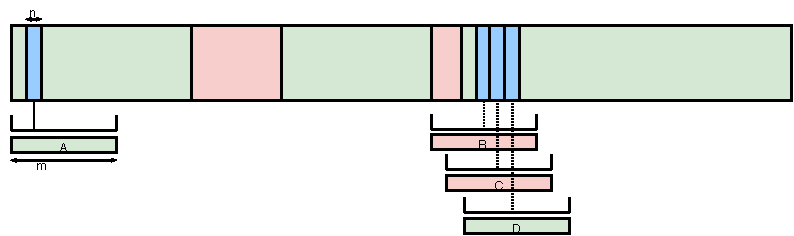
\includegraphics[width=\linewidth]{img/FocusBlocks}
	\caption{Process of splitting the whole code with vulnerable (red) and non vulnerable (green) parts in snippets for the dataset}
	\label{fig:FocusBlocks}
\end{figure}

The next step is to transform those code blocks, with are nothing more than lists of python tokens, into lists of numerical vectors. For this, we need the word2vec embedding. 

\subsection{Word2Vec embedding}
%python for training
To encode the code tokens in a word2vec vector, a fitting word2vec model is required that has been trained on python source code. To train this model, a large training base of code is required, ideally made up of clean, working Python code.\\
Similarly to ~\cite{Bhoopchand.2016} and ~\cite{Allamanis.2013}, I follow the  heuristic that popular code projects are of good quality. Note that those repositories are likely to contain few security vulnerabilities, as well as bugs in general. Github offers two metrics to assess popularity of a repository: stars (highlights similar to bookmarks set by users) and forks (copies for further development and experimentation in a personal project). Choosing python repositories with a high number of stars and forks, the following selection of example repositories is gathered:

\footnotesize
\begin{itemize}[noitemsep]
\item https://github.com/numpy/numpy
\item https://github.com/django/django
\item https://github.com/scikit-learn/scikit-learn
\item https://github.com/tensorflow/tensorflow
\item https://github.com/keras-team/keras
\item https://github.com/ansible/ansible
\item https://github.com/TheAlgorithms/Python
\item https://github.com/pallets/flask
\item https://github.com/ytdl-org/youtube-dl
\item https://github.com/pandas-dev/pandas
\item https://github.com/scrapy/scrapy
\item https://github.com/kennethreitz/requests
\item https://github.com/home-assistant/home-assistant
\item https://github.com/ageitgey/face\_recognition
\item https://github.com/emesik/mamona
\item https://github.com/progrium/notify-io
\item https://github.com/phoenix2/phoenix
\item https://github.com/odoo/odoo
\item https://github.com/ageitgey/face\_recognition
\item https://github.com/psf/requests
\item https://github.com/deepfakes/faceswap
\item https://github.com/XX-net/XX-Net
\item https://github.com/tornadoweb/tornado
\item https://github.com/saltstack/salt
\item https://github.com/matplotlib/matplotlib
\item https://github.com/celery/celery
\item https://github.com/binux/pyspider
\item https://github.com/miguelgrinberg/flasky
\item https://github.com/sqlmapproject/sqlmap
\item https://github.com/zulip/zulip
\item https://github.com/scipy/scipy
\item https://github.com/bokeh/bokeh
\item https://github.com/docker/compose
\item https://github.com/getsentry/sentry
\item https://github.com/timgrossmann/InstaPy
\item https://github.com/divio/django-cms
\item https://github.com/boto/boto
\end{itemize}
\normalsize
With the tool pydriller~\cite{Spadini.2018}, the python files in those repositories can be downloaded (see script \texttt{10python-for-training.py}). The resulting source code is simply concatenated to form one huge python code file. Then, another script (\texttt{11RemoveProblems.py}) is used to remove problems within this file, for example indentation errors. Now, the built in python tokenizer is used to split the code into python tokens (\texttt{11TokenizerPythoncode.py}). Comments are removed from the file, and new lines, indentations and tabs are normalized. At this point, there are two different ways to go ahead: string tokens could be kept as they are, or they could be replaced with a generic string token. Both versions are tested. Finally, the results are concatenated in one big python file (\texttt{11tokenizerMerge.py}).\\
Using the gensim implementation for python, the Word2Vec model is then trained on the corpus. Parameters of the word2vec model include the dimensionality of the resulting vectors, the minimum number of times a token has to appear in the corpus to include it in the model, and the training iterations. Several different parameter settings are tested and evaluated. To see whether a trained embedding is useful, there are basically two options: One can simply look at some tokens and their most similar tokens according to the model, and think about whether they seem to make sense, which is of course a subjective approach. And the model can be evaluated by looking at the final performance of the LSTM, which can only work reasonably well if the way the training data is embedded is sensible. By judging from the final performance of the full model, the embedding parameters can be evaluated.\\
The following table shows the embedding of a word2vec model that doesn't replace strings, has a minimum count of 1000, a vector size of 200 and 100 iterations. Displayed are some words in the vocabulary and their respective most similar other tokens, as determined by the cosine similarity. A cosine similarity of '1' would mean that the two tokens are identical or complete synonyms.

\footnotesize
\begin{center}
	\begin{tabular}{ |c|c|c|c|c| } 
		\hline
		\textbf{word} & \textbf{ most similar} &\textbf{ second most similar} & \textbf{third most similar}& \textbf{forth most similar}\\ 
		\hline
		\textbf{import} & from (0.42) & collections (0.34) & print\_function (0.32) & importerror (0.31)\\ 
		\textbf{true} & false (0.90) & module (0.35) & boolean (0.35) & none (0.34)\\  
		\textbf{while} & break (0.54)  & -= (0.39) & found (0.38) & continue (0.37) \\
		\textbf{if} & elif (0.78)  & and (0.75) & or (0.72) & assert (0.59) \\
		\textbf{try} & else (0.50)  & attributeerror (0.46) & keyerror (0.40) & pass (0.36) \\
		\textbf{in} & is (0.48)  & hasattr (0.46) & isinstance (0.40) & == (0.36) \\
		\textbf{+} & += (0.66)  & \% (0.48) & - (0.43) & * (0.43) \\
		\textbf{x} & y (0.73)  & z (0.40) & condition (0.32) & alpha (0.28) \\
		\textbf{[} & ] (0.49)  & 1 (0.46) & 0 (0.43) & '' (0.40) \\
		\textbf{str} & bool (0.48)  & tuple (0.48) & list (0.45) & repr (0.45) \\
		\textbf{count} & total (0.53)  & len (0.50) & max (0.44) & counter (0.42) \\
		\textbf{len} & count (0.50)  & split (0.39) & max (0.39) & num (0.38) \\
		\textbf{where} & select (0.41)  & find (0.38) & sum (0.35) & mask (0.34) \\
		\textbf{join} & write (0.55)  & append (0.55) & extend (0.52) & dirname (0.45) \\
		\textbf{split} & parts (0.50)  & strip (0.46) & rstrip (0.49) & append (0.43) \\
		\textbf{==} & ! (0.71)  & > (0.56) & < (0.56) & hasattr (0.43) \\
		\hline
	\end{tabular}
\end{center}
\normalsize

Note that for example the operator '==', used to test for equality, is most similar to other operators for comparison that result in a boolean outcome. In general, the similarities seem plausible and suggest that the word2vec model was able to learn something about the role of different python tokens, e.g. that true and false have a very similar functionality in code.\\ 

The parameters of the word2vec model are:
\begin{itemize}[noitemsep]
	\item leaving strings; or replacing strings
	\item training iterations: 10, 50 or 100
	\item minimum count: 10, 50, 100 or 1000
	\item vector dimensionality: 5, 10, 15, 30, 50, 75, 100, 150, 200, 300
\end{itemize}

Judging from other applications and default values, it is likely that for example a vector dimensionality below 30 will not be able to capture the semantics of python code tokens and will results in poor overall model performance. Also, 100 training iterations will probably not make much of a difference compared to 50. All of those parameters are tried out to find a configuration that works well for this application.

\subsection{Preparing the Data for Classification}
The collected data is still in the format of vulnerable and non vulnerable code snippets. The snippets are converted into a list of tokens (e.g. 'if', 'init', '2.3' or '+') and each of the token is replaced with its vector representation according to the Word2Vec model that was chosen. Each list of vectors is associated with their binary label, '0' meaning vulnerable and '1' meaning not vulnerable or unknown status. Refer to \texttt{51MakeBlocks.py} for the actual script.\\
70\% of the data is then randomly selected as a training set, 15\% are taken as a test set for validation, and 15\% are put aside for a final evaluation at the very end of the experiments. This is well in line with general practice in training neural networks as well as other works on similar tasks, for example, \cite{Russell.2018} split their dataset in 80\% training, 10\% validation and 10\% final test set, and \cite{Li.2018} used a split of 80-20 in train and test set. \\
The lists of vectors, each representing what was one code snippet, are truncated and padded to achieve an equal length of vectors per datapoint.

\subsection{Training the Long Short Term Memory Network}

\subsubsection{Architecture of the Model}

%LSTM, Dropout, Dense

%TODO

\begin{figure}[ht]
	\centering
	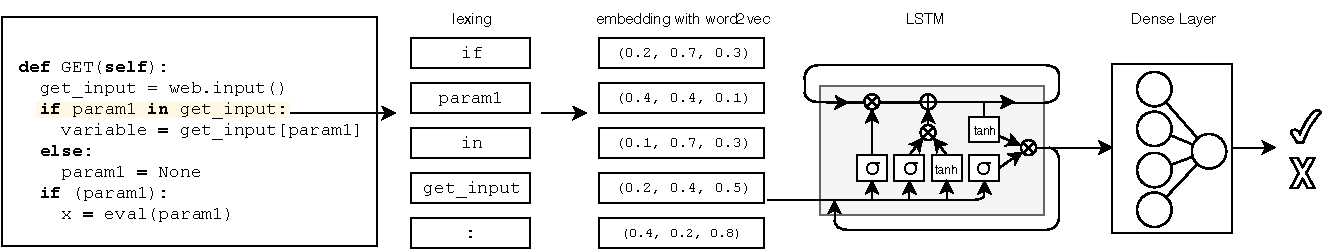
\includegraphics[width=\linewidth]{img/Architecture}
	\caption{architecture of the model}
	\label{fig:architecture}
\end{figure}

To implement the Long Short Term Memory network, the Keras library is used.\\
The main part is the Long-Short-Term-Memory layer, which has been described in its functionality in detail in section \ref{LSTM}. The purpose of this layer is to learn features which are associated with the vulnerability status of a code snippet. There is no seperate dropout layer, instead, there will be a dropout within the LSTM itself (see next section). The hyperparameters of the LSTM are subject to optimization.\\
After the LSTM layer, there is just the activation layer, in this case a dense output layer with a single neuron. The activation function used here is a sigmoid activation function because the goal is to make a prediction between 0 and 1 for the two classes of vulnerable or not vulnerable code. 


% The feature vector can then be used for measuring similarity between functions, predicting defects, checking for duplicates or, as in this case, to predict vulnerabilities~\cite{Dam.2017}.

%The LSTM layer is accompanied by a dropout layer. The purpos of this layer is to pick randomly selected neurons to ignore them during training, which reduces the tendency of the model to overfit. A dropout of 10-20\% is frequently used for a good balance between reducing overfitting and retaining accuracy.%TODO QUOTE https://towardsdatascience.com/choosing-the-right-hyperparameters-for-a-simple-lstm-using-keras-f8e9ed76f046

%TODO Try out with and without dropout


\subsubsection{Choosing Parameters}

A lot of decisions have to be made regarding the LSTM parameters.%TODO try out with and without weights
The first parameter is of course the number of \textbf{neurons} (or units). It affects the learning capacity, more neurons allowing the model to learn a more complex structure, but also requiring a longer time to train the model, and it is also the dimensionality of the output space.\\  
Since the data is inherently class-imbalanced (there are many more clean code blocks in the training data than vulnerable ones), the classes should be weighed accordingly. This assures that even though there are a lot more example for clean code, the examples for vulnerable code are taken just as seriously in training. The \textbf{class weights} are calculated automatically using the class\_weight function from the scikit-learn library.\\
\textbf{Metric and loss function} have to be adjusted to the goals of this work. Since a good balance between false positives and false negatives is desireable and the classes are already weighed, the F1 metric seems especially well suited to evaluate the overall performance (see section \ref{quantitative}). Therefore, the F1 score is chosen as the optimization criterium for the LSTM model. The F1 metric and the corresponding loss function are custom defined in the scripts.\\
The \textbf{batch size} desribes how many datapoints are shown to the network to be processed before the weights are updated again. Therefore, the model should not be trained with a batch size smaller than the number of datapoints used at a time when making a prediction later. A variety of different batch sizes are tried out to compare the results. The most extreme values would be a batch size of one single sample (as used in on-line learning or stochastik gradient descent approaches), or a batch size of a the full training set (batch forecasting). In the middle between the two, batch sizes of 32, 64 and 128 samples are typically used.\\
Like many models, LSTMs can trained to the point of overfitting training data, which reduces their predictive performance. \textbf{Dropout} is a regularization method where input and recurrent connections to LSTM units are sometimes randomly excluded from the next step of the training, so they can't be taken into account when the network updates its weights. This reduces the chance that the network overfits by relying on a few inputs too heavily. In LSTMs, there are two kinds of dropout: the standard dropout describes the fraction of units to drop from the inputs. The recurrent dropout describes the fraction of units to drop from the recurrent state (the memory of the previous steps of the model). A typical dropout is chosen between 10\% and 50\%. The ideal dropout will be determined by experimentation.\\
Finally, the \textbf{number of epochs}, in other words the number of times that the learning algorithm will work through the whole training data set, has to be adjusted. Typical numbers for epochs in literature include 10, 100, 500 or even 1000 epochs.\\

%metric, loss function, batch size, epochs


\subsubsection{Choosing the Optimizer}
%Li 2018 use Adamax
%Russel et al use Adam
%DAM 2017 use RMSprop
%LI and RUSSEL explain details about their parameters

A major consideration in training deep networks is the learning rate. Too small means the network won't learn quickly enough, too large means that the network won't deal well with a local minimum or an ill-conditioned region. With learning rate adaption, it is possible to modify the learning rate over the course of the learning process. One of the most popular algorithms for doing so is the Adam optimizer.\\
The Adam optimizer is an optimization algorithm for updating network weights that was published in 2014 \cite{Kingma.2014}
and is designed for deep neural networks and often achieves very good results fast. It computes individal learning rates for different parameters. According to the authors, it combines the advantages of the Adaptive Gradient Algorithm (Adagrad), which works well with sparse gradients~\cite{Duchi.2011}, and Root Mean Square Propagation (RMSprop), which adapts learning rates based on recent magnitudes of the gradients for the weight and performs well on on-line and non-stationary problems~\cite{Tieleman.2012}. The name is derived from 'adaptive moment estimation'. The Adam optimizer uses the first and second moment of the gradient, which are defined as the expected value of that variable to the power of one or two, respectively - those are the mean and the centered variance of the gradient. To estimate them, Adam uses exponetially moving averages, with two parameters beta1 and beta2 which control the decay rates of those moving averages. \\
For this project, the Adam optimizer is compared to three other popular optimizers: RMSProp, Adamax and Adagrad, and the best version is chosen.


\subsection{Application on code}
\includegraphics[width=0.5\textwidth]{img/Legende}\\
Finally, the usability of the trained classifier is tested on source code. The code is split in blocks in exactly the same way as before (using a small focus area and a sliding context window as described in section \ref{Processing}). The focus area traverses through the code, and for each new step the surrounding context is taken, the model makes a prediction based on that context as input, and the prediction is used as the vulnerability classification for the focus area. The following graphics illustrate this process in action. \\

\includegraphics[width=0.7\textwidth]{img/Example1}\\
\includegraphics[width=1\textwidth]{img/Example2}\\
\includegraphics[width=1\textwidth]{img/Example3}



\newpage

\section{Results}

\subsection{The baseline model}
To show the effects of various parameter changes and tweaks, a baseline model was created. Its parameters are not optimal, but it can be used to demonstrate how other parameters cause better or worse results, since some configuration has to be taken as a starting point. After going through all parameters and pointing out how they effect the final performance, the optimal combination of all paramters can be determined. The baseline model has a focus area step size n of 5, a context length m of 200, and works on the dataset for SQL injections. It has 50 neurons and is trained for 30 epochs with a dropout and recurrent dropout of 20\%, with a batch size of 200, using the adam optimizer. 

\subsection{Parameters and Performance of the Word2vec embedding}

The training corpus taken from various python repositories contains 69517343 (close to 70 million) individual token.

\subsubsection{Vector Length}
The code tokens are converted into numerical vectors of a certain length or dimensionality. The longer those vectors are, the more different 'axes' there are for putting words in relation to each other, allowing the word2vec model to capture more complex relationships. A vector size of less than 100 is unlikely to represent the semantics of python code well, judging from similar tasks with natural language, where vector sizes of 200 are typical.\\
To compare different vector lengths, the minimum count of a token to appear in the vocabulary is set to 1000 and training iterations of the word2vec model are set to 100. The model that replaces strings with a generic string token was used.



\begin{tabular}{| p{3.5cm}  | p{0.6cm} | p{0.6cm} | p{0.6cm} | p{0.6cm} | p{0.6cm} | p{0.6cm} | p{0.8cm} | p{0.8cm} | p{0.8cm} | p{0.8cm} | }
	\hline
	\textbf{Vector length:} & 5 & 10 & 15 & 30 & 50 & 75 & 100 & 150 & 200 & 300 \\
	\hline
	
	\textbf{F1 score:} & 29\% & 40\% & 54\% & 61\% & 60\% & 68\% & 67\% & 73\% & 78\% & 76\% \\
	\hline
	\hline
\end{tabular}

As is evident from the table, a reasonable vector size seems to be around 200. 


\subsubsection{String Replacement}

Strings occuring in the python training file could be replaced with a generic 'string' token, or they could be kept as they are. Replacing them might reduce the level of detail of the mode, but keeping them might put too much focus on the specific content of string tokens - it is hard to say beforehand what works better. To compare the two approaches, the number of iterations is fixed to 100 and the length of the embedding vectors is fixed to 200.

\begin{tabular}{ | p {3cm} | p{5cm} | p{5cm} | }
	\hline
\textbf{min\_count}	& \textbf{strings kept} & \textbf{strings replaced} \\
	\hline
	\textbf{10} & 64\% & 57\% \\
	\textbf{50} & 59\% & 62\% \\
	\textbf{300} & 59\% & 62\% \\
	\textbf{100} & 63\% & 59\% \\
	\textbf{500} & 63\% & 59\% \\
	\textbf{1000} &  64\% & 64\% \\
	\textbf{5000} & 63\% & 59\% \\
	\hline
	\hline
\end{tabular}

Judging by those results, there seems to be no strong advantage of one method over the other. Going forward, the version in which strings are replaced is the default choice.



\subsubsection{Minimum Count and Iterations}

The minimum count defines how often a token has to appear in the training corpus in order to actually get assigned a vector representation. Tokens that appear less often are simpyl ignored and will not be encoded (and instead skipped over later when whole lists of tokens are converted to lists of vectors). This is mostly to ignore rare variable names, strings or other identifiers that are not really relevant.\\
The number of iterations defines the number of repetitions in training the the word2vec model. It is to be expected that after a certain number of iterations, there will be no added benefit in further training.\\

\begin{tabular}{| p {2.5cm} |  p {1.6cm} | p {1.6cm} | p {1.6cm} | p {1.6cm} |p {1.6cm} | p {1.6cm} | }
\hline 
				    & \multicolumn{6}{c|}{Iterations}\\
\hline
\textbf{min\_count} &  \textbf{5} &  \textbf{10} &  \textbf{30} &  \textbf{100} &  \textbf{500} & \textbf{500}  \\	
\hline
\textbf{10} &  X & X & X & X  & X & X\\
\textbf{50} &  X & X & X & X  & X & X\\
\textbf{100} &  X & X & X & X & X & X \\
\textbf{300} &  X & X & X & X & X & X \\
\textbf{500} &  X & X & X & X & X & X \\
\textbf{1000} &  X & X & X & X  &  X & X\\
\textbf{5000} &  X & X & X & X  & X & X\\	
\hline
\hline

\end{tabular}

Looking at those results, it is determined that a mininum count of XY with Z iterations seems to be a reasonable choice going forward. With string replacedment and a vector size of 200, all the parameters for the word2vec model are now determined.

%\begin{tabular}{ | p {2.5cm} |  p {1.2cm} |  p {1.7cm} | p {1.2cm} | p {1.7cm} | p {1.2cm} | p {1.7cm} |}
%\hline
%\textbf{min\_count} & \multicolumn{2}{c|} {\textbf{10 iter.}} & \multicolumn{2}{c|} {\textbf{50 iter.}}  & \multicolumn{2}{c|} {\textbf{100 iter.}}   \\
%\hline
% & \textbf{kept} & \textbf{replaced} & \textbf{kept} & \textbf{replaced} & \textbf{kept} & \textbf{replaced} \\
%\hline
%\textbf{10} & 1 & 2 & 3 & 4 & 5 & 6 \\

%\hline


%\end{tabular}


%\begin{tabular}{ | p{2cm}| p{2cm} | p{2cm} || p{2cm}|p{2cm}|p{2cm}|p{2cm}|  }
%	\hline
%	\multicolumn{7}{|c|}{word2vec parameters and resulting metrics} \\
%	\hline
%	\multicolumn{3}{|c||}{word2vec parameters} & Accuracy & Precision & Recall & F1 \\
%	\hline
%	MinCount & Iterations & Strings & Accuracy & Precision & Recall & F1  \\
%	\hline
%	10 & 100 & replaced & 0.00 &  0.00 &  0.00 &  0.00  \\
%	50 & 50 & kept & 0.00 &  0.00 &  0.00 &  0.00  \\
%	100 & 50 & replaced & 0.00 &  0.00 &  0.00 &  0.00  \\
%	10 & 100 & kept & 0.00 &  0.00 &  0.00 &  0.00  \\
%	\hline
%	\hline
%\end{tabular}



\subsection{Comparison of LSTM Optimizers}

When evaluating different hyperparameters of the LSTM, the default values from the baseline model are still used for the parameters not in question. The word2vec model with the parameters determined before is now used for all experiments.

\subsubsection{Number of neurons}

TODO..


\begin{tabular}{ | p{2cm} || p{2cm}|p{2cm}|p{2cm}|p{2cm}|  }
	\hline
	Neurons & Accuracy & Precision & Recall & F1 \\
	\hline
	5 & 0.0 &  0.0 &  0.0 &  0.0 \\
	10 & 0.0 &  0.0 &  0.0 &  0.0 \\
	20 & 0.0 &  0.0 &  0.0 &  0.0 \\
	30 & 0.0 &  0.0 &  0.0 &  0.0 \\
	50 & 0.0 &  0.0 &  0.0 &  0.0 \\
	70 & 0.0 &  0.0 &  0.0 &  0.0 \\
	100 & 0.0 &  0.0 &  0.0 &  0.0 \\
	150 & 0.0 &  0.0 &  0.0 &  0.0 \\
	200 & 0.0 &  0.0 &  0.0 &  0.0 \\
	\hline
	\hline
\end{tabular}



\subsubsection{Batch size}

Using the baseline model, typical batch sizes (32, 64 and 128) and some batch sizes much smaller and much larger are tried.

\begin{tabular} { | p{3cm} || p{0.8cm} | p{0.8cm} |  p{0.8cm} | p{0.8cm}  | p{0.8cm} | p{0.8cm} | p{0.8cm}| p{0.8cm} |}
	\hline
	\textbf{Batch Size:}  & 1 & 10 & 32 & 64 & 128 & 200 & 500 & 1000\\   
	\hline
	\textbf{F1 score:} & X\% & X\% & X\% & X\% & X\% & X\% & X\% & X\% \\
	\hline
	\hline
\end{tabular}

The batch size doesn't seem to have a strong influence on the overall performance of the model. Henceforth, a batch size of 200 will be used.

\subsubsection{Dropout}

Dropout and recurrent dropout are chosen together. Since the baseline model is trained for 30 epochs, there are still some variations in the result that can account for a variance of around 2 percent points. The following results were obtained:

\begin{tabular} { | p{2cm} || p{0.8cm} | p{0.8cm} | p{0.8cm} | p{0.8cm}  | p{0.8cm} | p{0.8cm} | p{0.8cm} | p{0.8cm} | p{0.8cm} | p{0.8cm} | p{0.8cm} |}
\hline
\textbf{Dropout:}  & 0\% & 5\% & 10\% & 15\%   & 20\% & 25\% & 30\%   & 35\% & 40\% & 45\% & 50\% \\   
\hline
\textbf{F1 score:} & 70\% & 72\% & 71\% & 72\% & 69\% & 71\% & 65\% & 62\% & 60\% & 59\% & 56\% \\
\hline
\hline
\end{tabular}

There is a decline in performance occuring when the dropout is set to a fraction larger than 25\%. Therefore, it seems like a solid choice to set the default dropout to 20\%, preventing overfitting while still allowing for a strong model performance.



\subsubsection{Optimizer}

The optimizers Adam, Adamax, Adagrad, RMSProp and XYZ are compared. 

\begin{tabular}{ | p{2cm} || p{2cm}|p{2cm}|p{2cm}|p{2cm}|  }
	\hline
	Optimizer & Accuracy & Precision & Recall & F1 \\
	\hline
	Adam & 0.0 &  0.0 &  0.0 &  0.0 \\
	Adagrad & 0.0 &  0.0 &  0.0 &  0.0 \\
	Adamax & 0.0 &  0.0 &  0.0 &  0.0 \\
	RMSProp & 0.0 &  0.0 &  0.0 &  0.0 \\
	... & 0.0 &  0.0 &  0.0 &  0.0 \\
	\hline
	\hline
\end{tabular}


\subsubsection{Number of training epochs}

TODO..

\begin{tabular}{ | p{2cm} || p{2cm}|p{2cm}|p{2cm}|p{2cm}|  }
	\hline
	Epochs & Accuracy & Precision & Recall & F1 \\
	\hline
	5 & 0.0 &  0.0 &  0.0 &  0.0 \\
	10 & 0.0 &  0.0 &  0.0 &  0.0 \\
	20 & 0.0 &  0.0 &  0.0 &  0.0 \\
	30 & 0.0 &  0.0 &  0.0 &  0.0 \\
	50 & 0.0 &  0.0 &  0.0 &  0.0 \\
	70 & 0.0 &  0.0 &  0.0 &  0.0 \\
	100 & 0.0 &  0.0 &  0.0 &  0.0 \\
	150 & 0.0 &  0.0 &  0.0 &  0.0 \\
	200 & 0.0 &  0.0 &  0.0 &  0.0 \\
	\hline
	\hline
\end{tabular}

\subsubsection{Optimal configuration}


TODO..






\subsection{Performance for subsets of vulnerabilities}


TODO..

\begin{tabular}{ | p{5cm} || p{2cm}|p{2cm}|p{2cm}|p{2cm}|  }
	\hline
	Subset & Accuracy & Precision & Recall & F1 \\
	\hline
	SQL Injection & 0.0 &  0.0 &  0.0 &  0.0 \\
	Command Injection & 0.0 &  0.0 &  0.0 &  0.0 \\
	... & 0.0 &  0.0 &  0.0 &  0.0 \\
	\hline
	\hline
\end{tabular}



\newpage
\section{Discussion}


\subsection{Answers to Research Questions}

\subsubsection{Research Question 1}
\textbf{Can a dataset of suitable python source code be mined from Github for common vulnerability types?}


\subsubsection{Research Question 2}
\textbf{Is the word2vec model effective as an embedding, and how do its the parameters influence the overall results?}

\subsubsection{Research Question 3}
\textbf{Which types of vulnerabilities can be detected?}

\subsubsection{Research Question 4}
\textbf{How effective is VUDENC in detecting vulnerabilities as measured with accuracy, precision and recall? }


\subsection{Comparison with other works}

The following section contains comparisons with similar works in the field to provide a reference frame for the evaluation of this work. Of course, there are fundamental differences in each approach, and no direct comparison can be drawn.\\
Approaches are compared under the following aspects:\\
\begin{itemize}
	\item \textbf{Language:} what language is subject of the classification efforts
	\item \textbf{Data basis:} does the data stem from real-life projects or from synthetic databases (e.g. benchmark data sets).
	\item \textbf{Labels:} how are the labels for the training data originally generated
	\item \textbf{Granularity:} is the code evaluated on a rough granularity (e.g. whole classes or files) or a fine granularity (e.g. lines or tokens)
	\item \textbf{Machine Learning Approach:} what class of neural network or machine learning approach is used (e.g. CNN, RNN, LSTM)
	\item \textbf{Vulnerability types:} which kinds of vulnerabilities are detected
	\item \textbf{Size of data set:} how many functions, projects, classes etc. make up the dataset
	\item \textbf{Scope and applicability:} Has the model been trained on a single project and can it only classify files within that application, or is it generally applicable to any code from a large variety of sources
\end{itemize}


Russel et al. ~\cite{Russell.2018} worked directly on lexed source code and are very similar in their approach to what is presented here. They take C and C++ code from real software packages including Github and the Debian Linux distribution as well as from benchmark dataset to find vulnerabilities. Their dataset is impressively large with (e.g. 9 million functions from github). They use not exactly the same type of deep neural network, but similar CNN and RNN networks. The main difference is that they use static parsers to generate the labels, while the X approach relies only on commit contexts to create labels. They identify five different types of vulnerabilities, including buffer overflows and null pointers, which of course are quite different from the vulnerabilities found in python code. Russel et al. use a Random Forest classifier for the final classification step. On natural data sets, they achieve an F1 score of 0.566.\\

Pang et al. ~\cite{Pang.2015} use a hybrid n-gram and feature selection analysis on a dataset consisting of four Java android applications. The downloaded the labels from an online benchmark that was already prepared. They conduct their analysis on the level of whole classes (rough granularity) and try to predict whether the class contains a vulnerability or not by training a Support Vector Machine. While they achieve good results for prediction within the very same project (accuracy, precision and recall around 90 percent), the cross-project results are less strong with an F1 score of around 65\%. The two main differences here are that the X approach uses a much larger and more diverse data, and that the X approach can point out very specific locations in the code where a vulnerability might be, possibly being more useful to the developer in practise.\\

The tool VuRLE ~\cite{Ma.2017} was trained on 40 applications in Java collected from Github. The commits are analyzed manually to find vulnerabilities of five different types. Abstract syntax trees are the basis for the approach in which 'edit groups' are created to classify vulnerabilities, using 10-fold cross validation. Five different kinds of vulnerabilities are detected, including for example SQL injections. Although their main goal is to create repair templates, they first have to detect vulnerabilities, which they manage with an F1 score of around 65\%. \\

Li et al. ~\cite{Li.2018} developed the tool VulDeePecker to detect buffer error vulnerabilities and resource management error vulnerabilities in C/C++ programs. They work on a 'code gadget database' made from a large number of popular open source projects, including the linux kernel and Firefox. The vulnerabilities are found by using the NVD and SARD dataset, which contain synthetic and real life / production code, flaws and vulnerabilities. In selecting their data from those sources, Li et al work on very high-quality code. Just as the X approach, they use code changes / patches to find vulnerabilities and create their labels, but include a second step of human supervision to double check every positive label manually (in contrast, the X approach is completely automatic). They train a bidirectional LSTM and achieve an impressive F1 score of around 85-95\%. The X approach can not achieve a similarly high score since it uses data from all kinds of Github projects, which are not as clearly categorized and perfectly categorized as the high-profile projects which are used to train VulDeePecker. Furthermore, the database of the X approach only consists of real life code and no synthetic code.\\

The authors of VulDeePecker compare their tool other approaches and find a F1 score of 27\% for the tool Flawfinder, 47\% for Checkmarx, 18.2\% for VulPecker, and 9.3\% for VUDDY. The latter two, however, are optimized to have close to zero false positives.\\

The authors of ~\cite{Dam.2017} train a LSTM on 18 android applications. In an approach that is very similar to the X approach, they look at code tokens and represent them with multi-dimensional vectors, however, their feature extraction algorithm is focused on the specific project, learning relevant syntactic and semantic information that is specific for this one application. The only classify whole files, working on a very rough granularity. In their best configuration, they achieve an precision, recall and F1 measure of around 91\% - however, only for predictions within the \textit{same single} project on which the classifier was trained. For inter-project predictions, they do not present those metrics, but rather state the \textit{number} of other projects (out of 17) that a model trained on one project can classify with precision and recall of more than 80\%. On average, their models are able to classify the vulnerabilities in 4 out of 17 other projects.\\

~\cite{Hovsepyan.2012} et al. focus their efforts on one single Java application and try to predict whether a whole file is vulnerable or not. To this end, they split the file in tokens and use a static tool to create the labels for their files, and use a radial base function and a grid search algorithm to learn their features for the classification. They achieve an accuracy, precision and recall of over 80\%. It is unclear how useful those results are, given that they work only on this one single project, and they can not locate vulnerabilities, but only classify whole files. 

\scriptsize
\begin{tabular}{ | p{1.4cm} | p{1cm}|  p{0.8cm}| p{1.5cm} |  p{1.2cm} | p{1.5cm} | p{1.2cm} || p{0.4cm}|p{0.4cm}|p{0.4cm}|p{0.4cm}|  }
	\hline
	\multicolumn{7}{|c||}{characteristics of approach} & \multicolumn{4}{c|}{resulting metrics} \\
	%	\hline
	%	\multicolumn{3}{|c||}{word2vec parameters} & Accuracy & Precision & Recall & F1 \\
	\hline
	Name &  Language & Data & Labels & Scope &Granularity & Method & Acc. & Pre. & Rec. & F1  \\
	\hline
	Russel et al. & C/C++ & real \& synth. & static tool & general & token level (fine) & CNN, RNN &  &   &   &  57\%  \\
	\hline
	Pang et al. & Java & real  & pre-existing  & 4 apps & whole classes & SVM & 63\% & 67\%  & 63\%  & 65\%    \\
	\hline
	VuRLE & Java & real  & manually identified  & general & edits (fine) & 10-fold CV &  & 65\%  & 66\%  & 65\%    \\
	\hline
	VulDeePecker & C/C++ & real \& synth.  & patches \& manual & general & API/function calls & BLSTM &  &   &  & 85\%-95\%    \\
	\hline
	Dam et al. & Java & real &static tool & 18 apps & whole file & LSTM & \multicolumn{4}{c|}{ 4 / 17 (see above)}   \\
	\hline
	Hovsepyan et al. & Java & real  &static tool  & 1 project & whole file & grid search & 87\% & 	85\%  & 88\%  & 85\%   \\
	\hline
	X approach & Python & real  &patches& general  & token level & LSTM &  & &  &    \\
	\hline
	\hline 
\end{tabular}\\
\normalsize

In conclusion, we see that higher metrics in precision, recall and f1 are much easier to achieve if the approach focuses on preditions within a single project, as ~\cite{Hovsepyan.2012} and ~\cite{Dam.2017} do when they train a classifier to predict vulnerabilities within the very same application. Training a classifier that is applicable for general detection of vulnerabilities is much harder - but also much more interesting. Note that the same two approaches, as well as the one taken by  ~\cite{Pang.2015}, are also only trying to predict whether a whole file is vulnerable or not without being able to point out the exact location of the vulnerability. Since the X approach aims to develop a general vulnerability detector that can be used at the fine granularity of code tokens, it has a much more complicated task to fulfill.

Futhermore, the quality of a model depends a lot on the quality of the underlying data. Classification and prediction on synthetic data sets, or data sets that are curated and selected manually, will therefore be easier than training a model on possibly messy real life code from sources such as Github. With essentially the same approach, Russel et al. achieved 56\% on natural code from Github, but 84\% on the SATE test suite due to its clean and consistent style and structure. There, the X approach arguably performs quite well given that it works purely on natural real-life code. 







\subsection{Limitations and Threats to Validity}

\paragraph{Labeling based on the commit context}\mbox{}\\
A major threat to the external validity of this work is the reliance on commit contexts for classifying code snippets into vulnerable or (probably) not vulnerable. It is assumed that in general, there was an actual vulnerability, and the fixed version is in some way better than the previous versions. Of course, there are many situations in which those assumptions don't hold true, and as there is no other method of double-checking the vulnerability status applied in this work. The typical way do to this would be to chose a static analysis tool or bug checker, however, this work aims to work out the insights that can be gained without \textit{any} prior knowledge or pre-made assumptions about vulnerabilities, just using the code database a a source of information for the neural network. There might be a lot of undetected vulnerabilities in the files labeled as 'possibly not vulnerable' just because no developer ever fixed them, and our network can therefore also not learn to spot them. Furthermore, some fixes could be plain wrong. The answer to this problem is purely the size of the dataset, in which such retrictions might not play a big role compared to many legitimate fixes that share characteristics.
\paragraph{Systematic oversights due to developer decisions}\mbox{}\\
The dataset does only contain fixes that were actually applied by developers, and vulnerabilities that are either never detected or that developers chose to ignore remain invisible for the algorithm. This leads inevitably to blind spots in the classifier which retrict its ability to spot vulnerabilities. Note that \cite{Liu.2018} use exactly this restriction in their work \textit{on purpose}, as they are trying to learn which violations are actually fixed by developers and are therefore with some certainity not false positives. The situation is therefore ambivalent: false positives as they would result from using tools that report assumed violations are avoided better by only taking problems into account that were actually fixed. On the other hand, false negatives could be introduced for vulnerabilities that developers don't notice, understand or care about.
\paragraph{Limitations in types of vulnerabilities}\mbox{}\\
Altough a wide variety of different types of vulnerabilities was taken into account than in many other works, the list is of course not complete and the work focuses only on the most important and typical vulnerabilities. Therefore, rare and atypical kinds of vulnerabilities are not caught by the vulnerability detection.
\paragraph{Issues regarding the underlying data}\mbox{}\\
The data collected from Github might not be entirely representative of python source code in general. All data stems from projects that are publicly available on the platform, therefore the findings might not be applicable to industry and closed-source projects that might have different approaches reagarding code quality and spotting vulnerabilities. Furthermore, although we excluded projects that were marked as a fork on Github, it is very well possible that several projects in our database are very similar to each other. By the nature of open source and code sharing practises, some parts of the code in different repositories might even come close to being duplicates, meaning that the dataset is more limited than it first seems. Threats to internal validity include the fact that only python files were taken into account and e.g. XML files were ignored, although they might include security-relevant information. 
\paragraph{Unknown vulnerabilities}\mbox{}\\
The predictions are evaluated against known vulnerabilities in the past. A prerequisite for the model is the existence of vulnerabilities to learn from, and in cases where no known examples for code with vulnerabilities are available, this method cannot be applied. As pointed out by ~\cite{Yamaguchi.2012}, such situations are rare in practise, as the main concern for large software repositories is not to discover a single vulnerability, but to make sure that the same type of error does not spread across the project, which is what this method is useful for. Future vulnerabilities that are not yet known, or that developers are not aware of yet, can of course not be taken into account.
\paragraph{Not capturing the full context of a vulnerability}\mbox{}\\
The diff around a change provides that changed lines and three lines before and after them, respectively. There are certainly many situations in which a vulnerability steams from the interaction of lines of code that are spread out over a large file (or several files) and are interacting despite their distance from each other. However, the examples for vulnerabilities used to train the model only focus on the immediate surroundings of the fixed lines, and therefore, the model cannot learn the implications of far-reaching dependencies. However, the immediate surroundings of around 400-500 code tokens are most important to determine whether a code snippet contains a vulnerability. % TODO argue
\paragraph{Conclusion Vulnerability}\mbox{}\\
By using standard performance measures for the classifier that have been applied in other works regarding vulnerability prediction, threat to conclusion validity are minimized. To evaluate the performance of the predictions, accuracy, precision, and recall were used. However, in practice there may be other metrics and representation demonstrating how well a classifier performs.
\paragraph{Chosen method, model and parameters}\mbox{}\\
Threats to internal validity also include limitations in the chosen method. The basic prediction model used in this work is a LSTM, and as described at length in section \ref{Related-Work}, other models are used as well, such as CNNs, Naive Bayes and other. The results obtained from different models may vary. The data has been embedded using a Word2Vec model that was custom made for this application, and shortcomings in the Word2Vec model could affect the overall performance of the LSTM. Furthermore, some design decisions were, such as excluding occurrences of more than three seperators in a row, which might effect the overall end result.  
\paragraph{Relying on source code}\mbox{}\\
The present design of this work is limited to dealing with vulnerabilities in source code, for which such source code must be available. The detection of vulnerabilities in binary files or executables is a different problem that is not tackled here. 
\paragraph{Limitation in programming language}\mbox{}\\
The present version of the Word2Vec encoding used, the collection of files for training and testing the work, and the whole concept only focus on python code. While there is no specific reason why python should be more or less suitable for vulnerability detection than other languages that researchers in the field focus on (mainly C, C++, Java, PHP and Javascsript), this is undoubtedly a strong restriction of the model.


\subsection{Future Work}

\subsubsection{Different programming languages}

\subsubsection{}



\section{Conclusion}







\section{Bibliography}

\bibliographystyle{alpha}
\bibliography{bibliography,architectureopt}



\cleardoublepage% Wieder auf eine eigene Doppelseite
{\parindent0cm
	\subsection*{Selbständigkeitserklärung}
	Ich erkläre hiermit, dass ich die vorliegende Arbeit selbständig verfasst
	und noch nicht für andere Prüfungen eingereicht habe.
	Sämtliche Quellen einschließlich Internetquellen, die unverändert oder
	abgewandelt wiedergegeben werden, insbesondere Quellen für Texte, Grafiken,
	Tabellen und Bilder, sind als solche kenntlich gemacht. Mir ist bekannt,
	dass bei Verstößen gegen diese Grundsätze ein Verfahren wegen
	Täuschungsversuchs bzw. Täuschung eingeleitet wird.
	\vspace{3\baselineskip}
	
	%		\vspace{3\baselineskip}
	%
	% 		\selectlanguage{english}
	% 		\subsection*{Statement of authorship}
	% 		Hier würde die englische Selbständigkeitserklärung folgen, falls gewünscht. Doch es fehlt eine akzeptable Übersetzung.
	% 		\vspace{3\baselineskip}
	%
	% 		Berlin, #2 \hfill \TitelPunktLinie{6cm}
}




\end{document}


%note that...



%Due to the fundamental inability of one program to completely analyze another program's code, a generic technique for finding arbitrary vulnerabilities does not exist [10]. As a consequence, all practical approaches either limit the search to specific types of vulnerabilities or, as in the case of vulnerability extrapolation, only identify potentially vulnerable code.~\cite{Yamaguchi.2012}

%Unfortunately, the process of finding vulnerabilities cannot be automated in the general case. According to Rice's theorem a computer program is unable to generally decide whether another program contains vulnerable code~\cite{Yamaguchi.2012}


%oxford comma?